\documentclass[11pt,a4paper]{article}

\usepackage[margin=2.2cm]{geometry}
\usepackage[T1]{fontenc}
\usepackage{lmodern}
\usepackage{microtype}
\usepackage{amsmath,amssymb}
\usepackage{graphicx}
\usepackage{booktabs,tabularx,longtable,array}
\usepackage{xcolor}
\usepackage{enumitem}
\usepackage{float}
\usepackage{caption}
\usepackage{subcaption}
\usepackage{tikz}
\usepackage{pgfplots}
\usepackage[hidelinks]{hyperref}

\pgfplotsset{compat=1.18}
\usetikzlibrary{positioning,arrows.meta,shapes.geometric,shapes.multipart,fit,calc,backgrounds,matrix}

\definecolor{leaf}{HTML}{2F6B3B}
\definecolor{leafl}{HTML}{E6F0E3}
\definecolor{soil}{HTML}{3B2F24}
\definecolor{sand}{HTML}{F4EEE2}
\definecolor{turmeric}{HTML}{C98A1B}
\definecolor{sky}{HTML}{DCE8F3}
\definecolor{skyd}{HTML}{2E5E8C}
\definecolor{rose}{HTML}{F6E1DE}

\captionsetup{font=small,labelfont=bf}
\setlist{itemsep=2pt,topsep=4pt}
\graphicspath{{screenshots/}}
\renewcommand{\arraystretch}{1.18}
\newcolumntype{L}{>{\raggedright\arraybackslash}X}

% Diagram styles
\tikzset{
  box/.style={draw=leaf, fill=leafl, thick, minimum height=9mm, minimum width=26mm, align=center, font=\small},
  sbox/.style={draw=leaf, fill=white, thick, minimum height=7mm, minimum width=22mm, align=center, font=\footnotesize},
  ext/.style={draw=skyd, fill=sky, thick, minimum height=9mm, minimum width=26mm, align=center, font=\small},
  store/.style={draw=soil, fill=sand, thick, cylinder, shape border rotate=90, aspect=0.22, minimum height=13mm, minimum width=24mm, align=center, font=\small},
  actor/.style={draw=soil, fill=white, thick, rounded corners=0pt, minimum height=8mm, minimum width=22mm, align=center, font=\small},
  arr/.style={-{Stealth[length=2.4mm]}, thick, color=soil},
  darr/.style={{Stealth[length=2.4mm]}-{Stealth[length=2.4mm]}, thick, color=soil},
  lbl/.style={font=\scriptsize, fill=white, inner sep=1.5pt},
  zone/.style={draw=gray!60, dashed, inner sep=4mm},
  state/.style={draw=leaf, fill=leafl, thick, minimum height=8mm, minimum width=24mm, align=center, font=\small},
  bad/.style={draw=red!60!black, fill=rose, thick, minimum height=8mm, minimum width=24mm, align=center, font=\small},
}

% Pseudocode: a ruled float with numbered lines (no extra packages needed)
\floatstyle{ruled}
\newfloat{algorithm}{tbp}{loa}
\floatname{algorithm}{Algorithm}
\newenvironment{pseudo}{\small\begin{enumerate}[label={\scriptsize\arabic*}, leftmargin=7mm, itemsep=1pt, topsep=3pt]}{\end{enumerate}}
\newcommand{\kw}[1]{\textbf{#1}}
\newcommand{\ind}{\hspace*{5mm}}

\newcommand{\shot}[3][0.95]{%
  \begin{figure}[H]\centering
  \fbox{\includegraphics[width=#1\linewidth]{#2}}
  \caption{#3}\end{figure}}

\title{\textbf{Khet Se}\\[4pt]\large A Geo-Spatial Farm-to-Consumer Marketplace\\[2pt]\normalsize System Design Report}
\author{Ashutosh Choubey}
\date{}

\begin{document}
\maketitle

\begin{abstract}
\noindent Khet Se (``from the farm'') connects small organic farmers directly with households in the same city. Customers find produce from farms whose delivery area reaches them, ranked by distance, freshness, price, rating and organic certification. One checkout can span several farms. Each farmer fulfils their own part, and a farmer may hand the delivery to a Khet Se delivery partner, who picks the parcel up and hands it over against the customer's one-time code. An admin console verifies farmers, manages people, orders and refunds, and records every decision in an audit trail.

This report describes the system from a design perspective: requirements and capacity estimates, the architecture (the largest part), the algorithms with their reasons, the functionality as built, and how correctness and performance were verified. The system is deployed and serves a Raipur and Durg--Bhilai demo data set.
\end{abstract}

\tableofcontents
\newpage

%======================================================================
\section{Problem and Goals}
%======================================================================

Urban households in Tier-2 Indian cities want fresh, chemical-free vegetables and know that many such farms exist within 20--30\,km. They have no direct way to find or order from them. Small farmers sell through mandis and middlemen, lose a large share of the price, and cannot reach nearby customers. Khet Se is a city-scale marketplace that closes this gap.

\paragraph{Design goals.}
\begin{enumerate}
  \item \textbf{Location is the primary key of the product.} Everything a customer sees depends on where they are: which farms deliver to them, how far, how fresh and how expensive.
  \item \textbf{Never sell what does not exist.} Stock is held for an order the moment it is placed. Two buyers can never get the same last kilogram, and expired produce is never offered.
  \item \textbf{Each farm fulfils independently.} One basket may span three farms. Every farm accepts, packs and delivers its own part, and a failure at one farm must not block the others.
  \item \textbf{Four distinct users, one platform:} customers, farmers, delivery partners and administrators, each with their own workflows and strict data boundaries.
  \item \textbf{Run on modest hardware at launch, with a clear path to scale.} A single city should run on one machine; growth should mean adding processes, not rewriting.
\end{enumerate}

%======================================================================
\section{Requirements}
%======================================================================

\subsection{Functional requirements}

\begin{table}[H]\centering\small
\begin{tabularx}{\linewidth}{@{}p{2.7cm}L@{}}
\toprule
\textbf{Actor} & \textbf{Capabilities} \\
\midrule
Customer & Sign up and log in with mobile number and password (email optional); set a delivery location; browse nearby produce and farms with search, filters and sorting; cart across farms with live server pricing; checkout (cash on delivery or online); track each farm's part; see the delivery partner; hand over with a 4-digit code; cancel before acceptance; reset a forgotten password. \\
Farmer & Profile and organic certificate; farm with map location and delivery radius; listings with price, stock, harvest or expiry dates; incoming-order queue with acceptance deadline; accept, pack, deliver (with the customer's code) or request a delivery partner; see verification decisions and reasons. \\
Delivery partner & Vehicle, base location and work area; go online or offline; job board of open deliveries near the base; accept (first wins), pick up, hand over with the customer's code; earnings and cash collected. \\
Administrator & Platform overview; farmer profile and organic verification; people search, suspension and reactivation; order search, cancelling one farm's part, recording refunds; transactions; immutable audit trail. \\
\bottomrule
\end{tabularx}
\caption{Functional requirements by actor.}
\end{table}

\subsection{Non-functional requirements}

\begin{table}[H]\centering\small
\begin{tabularx}{\linewidth}{@{}p{3.2cm}L@{}}
\toprule
\textbf{Quality} & \textbf{Target and how it is met} \\
\midrule
Latency & Reads $p95 \le 300$\,ms and writes $p95 \le 800$\,ms at launch peak. Met with index-backed geo queries, batched joins, a short-lived result cache and pre-computed denormalised fields. \\
Correctness & No overselling, no double assignment of a delivery job, no order processed twice. Met with atomic conditional updates, multi-document transactions and idempotency keys. \\
Consistency & Search, product pages and checkout apply one shared ``sellable'' rule, so what is shown can always be ordered. \\
Security & Short-lived access tokens, rotating refresh tokens with theft detection, role-based access, per-IP rate limits, input validation, hashed secrets, audited admin actions, database bound to localhost with authentication. \\
Availability & Process supervision with automatic restart; graceful shutdown; background jobs that tolerate external outages. \\
Scalability & Stateless API processes; shared state only in MongoDB (and optionally Redis); the city is the natural shard key. \\
Usability & Works on low-end phones (mobile-first layouts, native controls); Hindi and local names for produce; clear reasons for every refusal. \\
\bottomrule
\end{tabularx}
\caption{Non-functional requirements.}
\end{table}

\subsection{Capacity estimation (one-city launch)}

\begin{table}[H]\centering\small
\begin{tabular}{@{}lrl@{}}
\toprule
\textbf{Quantity} & \textbf{Value} & \textbf{Basis} \\
\midrule
Daily active customers & 5{,}000 & $\approx 0.5\%$ of a Tier-2 urban population \\
Customer sessions per day & 8{,}000 & 1.6 sessions per active customer \\
Orders per day & 1{,}000 & 12.5\% of sessions convert \\
Farm parts (groups) per order & 1.4 & most baskets come from one or two farms \\
Active farmers & 200 & about 5 orders per farmer per day \\
Peak hour share & 14\% & evening grocery peak (7--9\,pm) \\
Peak customer sessions & 18.7 / min & $8000 \times 0.14 / 60$ \\
Peak orders & 140 / h & $1000 \times 0.14$ \\
Partner jobs at peak & 98 / h & $140 \times 1.4 \times 50\%$ delivered by partners \\
\bottomrule
\end{tabular}
\caption{Back-of-the-envelope load for the launch city.}
\end{table}

\noindent \textbf{Storage.} An order with two farm parts and history is about 3\,KB, so 1{,}000 orders a day is about 1\,GB a year with indexes. Listings, farms and users are small (tens of MB). One MongoDB replica set comfortably holds several cities for years. \textbf{Traffic.} Polling dominates: 60 partners refreshing the job board every 15--25\,s and 200 farmers checking orders every 60--120\,s produce more requests than shoppers. This shaped the choice of cheap, index-only queries for those screens (Section~\ref{sec:eval}).

%======================================================================
\section{System Architecture}
%======================================================================

\subsection{Architectural style}

Khet Se is a \textbf{modular monolith}: one API service whose code is split into well-separated modules (identity, catalogue, discovery, ordering, payments, delivery, administration). It sits behind one web application and uses one database.

\paragraph{Why not microservices?} The domain is tightly coupled at its core: placing an order reads listings, reserves stock, writes the order and records the payment, all in one transaction. Splitting these into services would replace a local ACID transaction with a distributed saga, adding failure modes (partial reservations, compensating messages) without benefit at city scale. A modular monolith keeps that transaction local, deploys as one unit, and still lets modules be extracted later along the boundaries in Table~\ref{tab:modules} if one of them needs to scale independently.

\paragraph{Why a separate web application?} The web front end (Next.js) and the API (Express) are separate projects and processes. The API is the single source of truth and is usable by any client (a future mobile app, partner integrations). The web tier can be scaled, cached or moved to a CDN without touching business logic.

\subsection{System context}

\begin{figure}[H]\centering
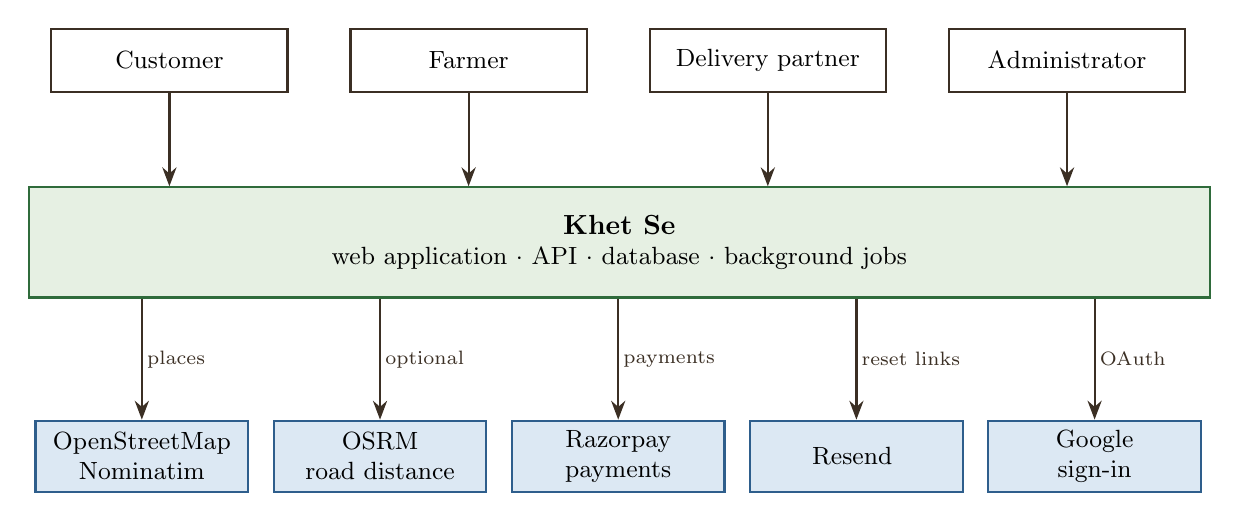
\begin{tikzpicture}[node distance=9mm and 10mm]
  \node[box, minimum width=150mm, minimum height=14mm, font=\normalsize] (sys) {\textbf{Khet Se}\\[-1pt]\small web application $\cdot$ API $\cdot$ database $\cdot$ background jobs};
  \foreach \i/\n/\t in {0/cust/Customer, 1/farm/Farmer, 2/part/Delivery partner, 3/adm/Administrator}
    \node[actor, minimum width=30mm] (\n) at ($(sys.north west)+(18mm+\i*38mm,16mm)$) {\t};
  \foreach \a in {cust,farm,part,adm} \draw[arr] (\a) -- (\a |- sys.north);
  \foreach \i/\n/\t/\l in {0/osm/OpenStreetMap\\Nominatim/places, 1/osrm/OSRM\\road distance/optional, 2/rzp/Razorpay\\payments/online orders, 3/mail/Resend / Brevo\\email/reset links, 4/goog/Google\\sign-in/OAuth}
    \node[ext, minimum width=27mm] (\n) at ($(sys.south west)+(14.5mm+\i*30.25mm,-20mm)$) {\t};
  \foreach \e/\l in {osm/places, osrm/optional, rzp/payments, mail/reset links, goog/OAuth}
    \draw[arr] (sys.south -| \e) -- node[lbl,right]{\l} (\e);
\end{tikzpicture}
\caption{System context: four kinds of users and the external services Khet Se depends on. All external services are optional or degrade gracefully; only the database is essential.}
\label{fig:context}
\end{figure}

\subsection{Deployment architecture}

\begin{figure}[H]\centering
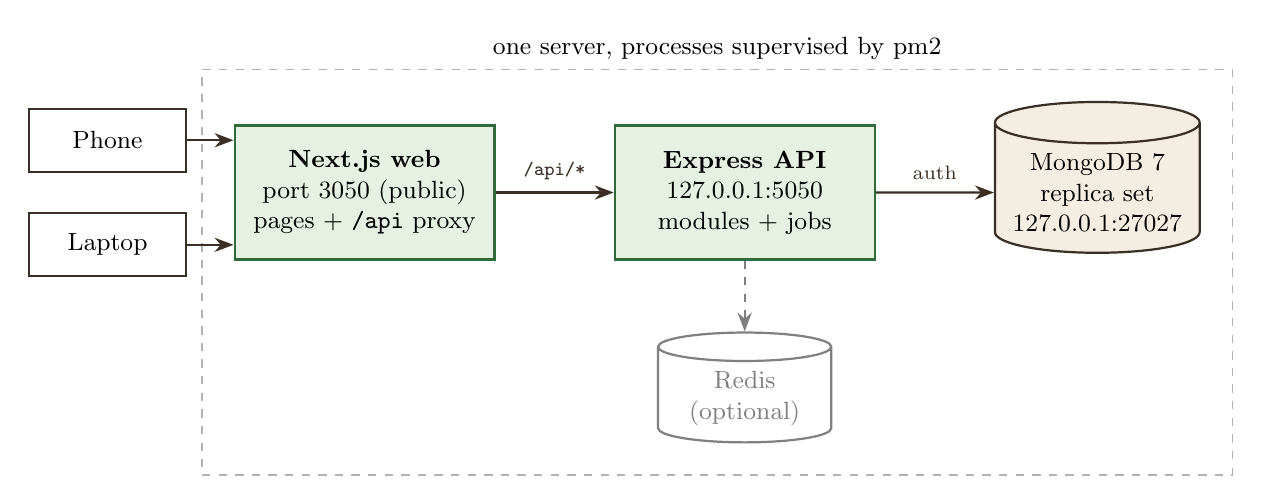
\begin{tikzpicture}[node distance=6mm and 14mm]
  \node[actor, minimum width=20mm] (b1) {Phone};
  \node[actor, minimum width=20mm, below=5mm of b1] (b2) {Laptop};
  \node[box, minimum width=33mm, minimum height=17mm, right=16mm of $(b1)!0.5!(b2)$] (web) {\textbf{Next.js web}\\port 3050 (public)\\pages + \texttt{/api} proxy};
  \node[box, minimum width=33mm, minimum height=17mm, right=15mm of web] (api) {\textbf{Express API}\\127.0.0.1:5050\\modules + jobs};
  \node[store, minimum width=26mm, minimum height=19mm, right=15mm of api] (db) {MongoDB 7\\replica set\\127.0.0.1:27027};
  \node[store, minimum width=22mm, below=9mm of api, fill=white, draw=gray, text=gray] (redis) {Redis\\(optional)};
  \draw[arr] (b1.east) -- (web.west |- b1.east);
  \draw[arr] (b2.east) -- (web.west |- b2.east);
  \draw[arr] (web) -- node[lbl,above=1mm]{\texttt{/api/*}} (api);
  \draw[arr] (api) -- node[lbl,above=1mm]{auth} (db);
  \draw[arr, gray, dashed] (api) -- (redis);
  \begin{scope}[on background layer]
    \node[zone, fit=(web)(api)(db)(redis), label={[font=\small]above:one server, processes supervised by pm2}] {};
  \end{scope}
\end{tikzpicture}
\caption{Deployment. Only the web server's port is reachable from the network. It serves pages and proxies \texttt{/api}, so the browser talks to one origin. The API and the database listen on localhost only; the database requires authentication.}
\label{fig:deploy}
\end{figure}

\paragraph{Why proxy the API through the web server?} A single origin removes cross-site cookie and CORS edge cases. It means only one port is exposed, and it lets the API trust exactly one proxy hop to read the client's real IP for rate limiting. The API remains independently addressable on the server for scripts and jobs.

\paragraph{Process model.} pm2 supervises three processes (\texttt{khetse-mongo}, \texttt{khetse-api}, \texttt{khetse-web}) with automatic restart, memory limits and log files. The runtime (Node 20, MongoDB 7, pm2) lives in a self-contained environment folder, so the deployment needs no system-wide installation or administrator rights. Secrets (database passwords, JWT secret) are generated on the server into a file only the service account can read. Updating is one script: fetch, build, sync indexes, restart.

\subsection{Back-end layered architecture}

\begin{figure}[H]\centering
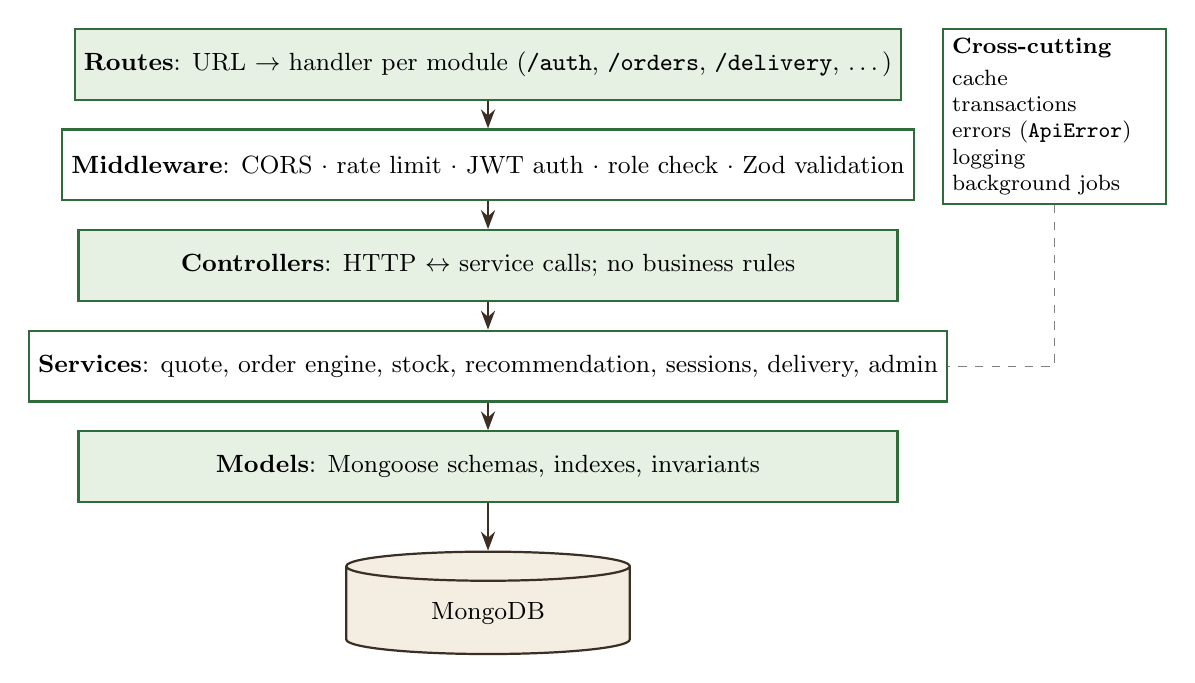
\begin{tikzpicture}[node distance=3.5mm, lay/.style={box, minimum width=104mm}]
  \node[lay] (r) {\textbf{Routes}: URL $\to$ handler per module (\texttt{/auth}, \texttt{/orders}, \texttt{/delivery}, \dots)};
  \node[lay, below=of r, fill=white] (m) {\textbf{Middleware}: CORS $\cdot$ rate limit $\cdot$ JWT auth $\cdot$ role check $\cdot$ Zod validation};
  \node[lay, below=of m] (c) {\textbf{Controllers}: HTTP $\leftrightarrow$ service calls; no business rules};
  \node[lay, below=of c, fill=white] (sv) {\textbf{Services}: quote, order engine, stock, recommendation, sessions, delivery, admin};
  \node[lay, below=of sv] (d) {\textbf{Models}: Mongoose schemas, indexes, invariants};
  \node[store, below=6mm of d, minimum width=36mm] (db) {MongoDB};
  \foreach \x/\y in {r/m,m/c,c/sv,sv/d,d/db} \draw[arr] (\x) -- (\y);
  \node[sbox, text width=26mm, minimum width=28mm, align=left, anchor=north west] (x) at ($(r.north east)+(5mm,0)$) {\textbf{Cross-cutting}\\[2pt] cache\\ transactions\\ errors (\texttt{ApiError})\\ logging\\ background jobs};
  \draw[gray, dashed] (x.south) -- (x.south |- sv.east) -- (sv.east);
\end{tikzpicture}
\caption{Request path through the API. Each layer depends only on the one below it, so services can be tested without HTTP and swapped behind the same routes.}
\end{figure}

\noindent Errors are raised as typed \texttt{ApiError}s (status, machine-readable code, message, field details) and turned into one response shape by a central handler: \texttt{\{success, data, meta\}} or \texttt{\{success:false, error:\{code, message, details\}\}}. Every input is validated by a Zod schema before reaching a controller, and the parsed (coerced, trimmed, defaulted) value replaces the raw input. For example, mobile numbers in any written form become 10 digits.

\subsection{Module decomposition}

\begin{table}[H]\centering\small
\begin{tabularx}{\linewidth}{@{}p{3.1cm}Lp{3.4cm}@{}}
\toprule
\textbf{Module} & \textbf{Responsibility} & \textbf{Owns} \\
\midrule
Identity \& sessions & Sign-up and login (mobile or email), refresh-token rotation, logout everywhere, password reset, Google OAuth & users, sessions, passwordresets \\
Catalogue & Shared product definitions (name, type, shelf life, category); cached in memory & products \\
Farmer \& farm & Farmer profile, organic certificate, farm location and delivery radius & farmers, farms \\
Inventory & Farmer listings: price, unit, stock, dates; denormalised farm location & inventory \\
Discovery & Geo retrieval, eligibility, scoring, diversity, radius widening, result cache & (reads) \\
Quote \& order engine & Server-side pricing, delivery fees, stock reservation, order state machine, idempotency & orders \\
Payments & Cash-on-delivery records, Razorpay orders, signature checks, reconciliation & payments \\
Delivery & Delivery records per farm part, partner profiles, job board, claims, handover & deliveries, deliverypartners \\
Administration & Overview, verification, suspensions, admin cancel, refunds, audit & adminactions \\
Geo & Place search and reverse geocoding (proxied, cached, throttled) & (external) \\
Jobs & Expire unpaid orders, expire unaccepted orders, reconcile payments, audit reserved stock & (schedules) \\
\bottomrule
\end{tabularx}
\caption{Modules and their boundaries. Each module's collections are written only by that module's services.}
\label{tab:modules}
\end{table}

\subsection{Front-end architecture}

The web application uses the Next.js App Router with route groups per audience: \texttt{(shop)} for customers and guests, \texttt{(auth)} for sign-in pages, and \texttt{/farmer}, \texttt{/delivery} and \texttt{/admin} for the three dashboards. The three dashboards share one layout component (sidebar on desktop, scrolling tab bar on phones). A client-side guard redirects to login or explains which role a page needs; the API enforces the same rules independently.

\begin{figure}[H]\centering
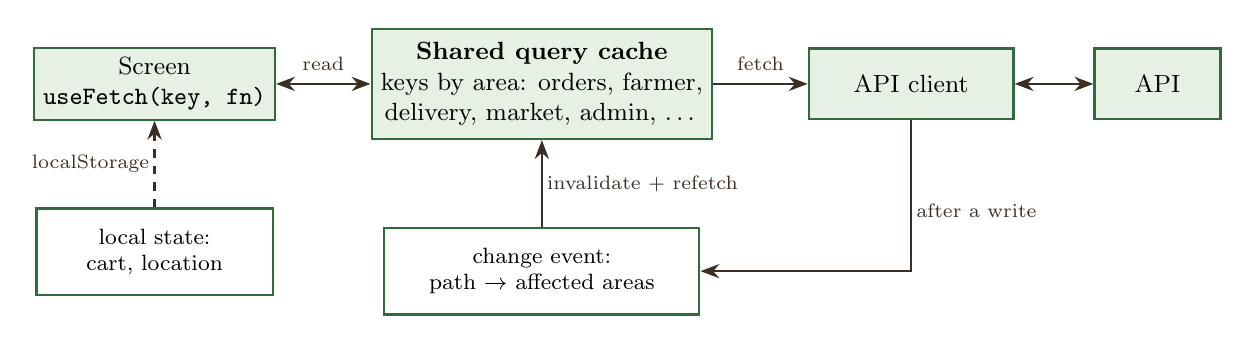
\begin{tikzpicture}[node distance=7mm and 12mm]
  \node[box, minimum width=30mm] (screen) {Screen\\\texttt{useFetch(key, fn)}};
  \node[box, right=of screen, minimum width=40mm, minimum height=14mm] (cache) {\textbf{Shared query cache}\\keys by area: orders, farmer,\\delivery, market, admin, \dots};
  \node[box, right=of cache, minimum width=26mm] (client) {API client};
  \node[box, right=10mm of client, minimum width=16mm] (api) {API};
  \node[sbox, below=11mm of cache, minimum width=40mm, minimum height=11mm] (bus) {change event:\\path $\to$ affected areas};
  \node[sbox, below=11mm of screen, minimum width=30mm, minimum height=11mm] (local) {local state:\\cart, location};
  \draw[darr] (screen) -- node[lbl,above=1mm]{read} (cache);
  \draw[arr] (cache) -- node[lbl,above=1mm]{fetch} (client);
  \draw[darr] (client) -- (api);
  \draw[arr] (client.south) |- node[lbl,pos=0.3,right]{after a write} (bus.east);
  \draw[arr] (bus) -- node[lbl,right]{invalidate + refetch} (cache);
  \draw[arr, dashed] (local) -- node[lbl,left]{localStorage} (screen);
\end{tikzpicture}
\caption{Client data flow. Screens never reload by hand: every successful write announces its path, the cache invalidates the areas it can affect, and every visible screen showing those areas refetches.}
\label{fig:clientdata}
\end{figure}

\paragraph{Design decisions.}
\begin{itemize}
  \item \textbf{One shared cache (TanStack Query) instead of per-screen fetching.} Screens with the same key share one request and always show the same data. The cache refetches when the user returns to the tab, and polls where people wait for new work: the farmer's order queue (30\,s), the partner job board (20\,s) and the customer's order page (30\,s).
  \item \textbf{Path-to-area invalidation.} For example, \texttt{PUT /orders/:id/status} invalidates \emph{orders, farmer, delivery, inventory, market, admin}. This replaces ad-hoc reload calls and guarantees that an action in one place (accepting an order) refreshes dependent views (dashboard counts, stock).
  \item \textbf{Account isolation.} The whole cache is cleared whenever the signed-in account changes. A session lost elsewhere (logout on another device, suspension) is shown as logged out instead of as errors.
  \item \textbf{Silent session renewal.} A 401 triggers one shared refresh call (single-flight), then the original request is retried once.
  \item \textbf{Local-only state.} The cart and delivery location are kept in the browser; the cart is always re-priced by the server.
\end{itemize}

\subsection{Data model}

\begin{figure}[H]\centering
\resizebox{\linewidth}{!}{%
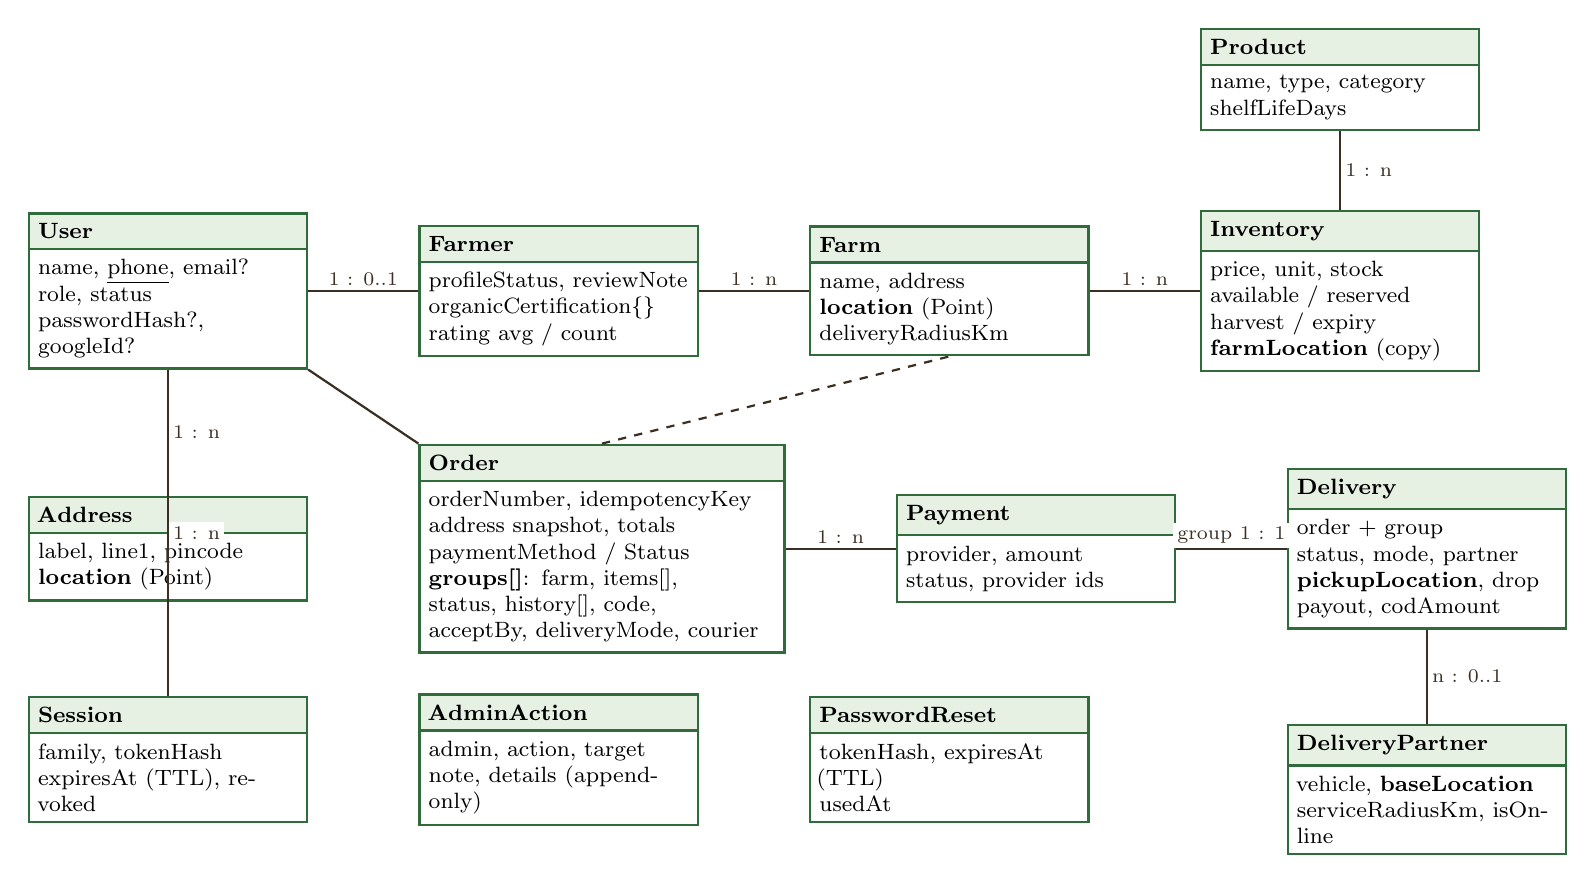
\begin{tikzpicture}[node distance=10mm and 14mm,
  ent/.style={draw=leaf, thick, rectangle split, rectangle split parts=2, rectangle split part fill={leafl,white}, font=\footnotesize, align=left, minimum width=34mm, text width=33mm},
  rel/.style={thick, color=soil}]
  \node[ent] (user) {\textbf{User}\nodepart{two}name, \underline{phone}, email?\\role, status\\passwordHash?, googleId?};
  \node[ent, right=of user] (farmer) {\textbf{Farmer}\nodepart{two}profileStatus, reviewNote\\organicCertification\{\}\\rating avg / count};
  \node[ent, right=of farmer] (farm) {\textbf{Farm}\nodepart{two}name, address\\\textbf{location} (Point)\\deliveryRadiusKm};
  \node[ent, right=of farm] (inv) {\textbf{Inventory}\nodepart{two}price, unit, stock\\available / reserved\\harvest / expiry\\\textbf{farmLocation} (copy)};
  \node[ent, above=of inv] (prod) {\textbf{Product}\nodepart{two}name, type, category\\shelfLifeDays};

  \node[ent, below=16mm of user] (addr) {\textbf{Address}\nodepart{two}label, line1, pincode\\\textbf{location} (Point)};
  \node[ent, right=of addr, text width=44mm, minimum width=45mm] (order) {\textbf{Order}\nodepart{two}orderNumber, idempotencyKey\\address snapshot, totals\\paymentMethod / Status\\\textbf{groups[]}: farm, items[],\\status, history[], code,\\acceptBy, deliveryMode, courier};
  \node[ent, right=of order] (pay) {\textbf{Payment}\nodepart{two}provider, amount\\status, provider ids};
  \node[ent, right=of pay] (del) {\textbf{Delivery}\nodepart{two}order + group\\status, mode, partner\\\textbf{pickupLocation}, drop\\payout, codAmount};

  \node[ent, below=12mm of del] (dp) {\textbf{DeliveryPartner}\nodepart{two}vehicle, \textbf{baseLocation}\\serviceRadiusKm, isOnline};
  \node[ent, below=12mm of addr] (sess) {\textbf{Session}\nodepart{two}family, tokenHash\\expiresAt (TTL), revoked};
  \node[ent, right=of sess] (aa) {\textbf{AdminAction}\nodepart{two}admin, action, target\\note, details (append-only)};
  \node[ent, right=of aa] (pr) {\textbf{PasswordReset}\nodepart{two}tokenHash, expiresAt (TTL)\\usedAt};

  \draw[rel] (user) -- node[lbl,above]{1 : 0..1} (farmer);
  \draw[rel] (farmer) -- node[lbl,above]{1 : n} (farm);
  \draw[rel] (farm) -- node[lbl,above]{1 : n} (inv);
  \draw[rel] (prod) -- node[lbl,right]{1 : n} (inv);
  \draw[rel] (user) -- node[lbl,right]{1 : n} (addr);
  \draw[rel] (user.south east) -- (order.north west);
  \draw[rel] (order) -- node[lbl,above]{1 : n} (pay);
  \draw[rel] (pay) -- node[lbl,above]{group 1 : 1} (del);
  \draw[rel] (del) -- node[lbl,right]{n : 0..1} (dp);
  \draw[rel, dashed] (order.north) -- (farm.south);
  \draw[rel] (user) -- node[lbl,right]{1 : n} (sess);
\end{tikzpicture}}
\caption{Data model (MongoDB collections). Points are GeoJSON with 2dsphere indexes. An order embeds its farm parts (\emph{groups}) because they are always read and updated with the order; unbounded data (listings, orders, sessions) lives in its own collections.}
\label{fig:er}
\end{figure}

\paragraph{Embedding versus referencing.}
\begin{itemize}
  \item \textbf{Embedded:} an order's farm parts, item snapshots, status history and the address snapshot. They belong to the order, are bounded in size and must change atomically with it. Item prices are \emph{snapshots}, so later price edits never alter past orders.
  \item \textbf{Referenced:} listings, farms, payments, deliveries and sessions. They grow without bound, are queried on their own (job board, admin lists) or have their own life cycle.
  \item \textbf{Denormalised copies:} \texttt{Inventory.farmLocation} copies the farm's point, so a single \texttt{\$geoNear} over listings finds products near a customer without a join. It is re-synced whenever a farm moves, and the algorithm checker verifies it (Section~\ref{sec:eval}). \texttt{Order.groups.courier} snapshots the partner's name, phone and vehicle for display.
\end{itemize}

\begin{table}[H]\centering\small
\begin{tabularx}{\linewidth}{@{}p{3cm}p{5.4cm}L@{}}
\toprule
\textbf{Collection} & \textbf{Index} & \textbf{Serves} \\
\midrule
inventory & \texttt{farmLocation: 2dsphere} & product discovery (\texttt{\$geoNear}) \\
farms & \texttt{location: 2dsphere} & farm discovery, checkout distances \\
deliveries & \texttt{pickupLocation: 2dsphere, status} & partner job board \\
deliveries & \texttt{partner, status, updatedAt} & a partner's own jobs \\
orders & \texttt{customer, idempotencyKey} (unique) & duplicate-submission protection \\
orders & \texttt{groups.farmer, groups.status, createdAt} & farmer order queues \\
orders & \texttt{groups.status, groups.acceptBy} & acceptance-deadline job \\
orders & \texttt{paymentStatus, reservationExpiresAt} & unpaid-order expiry job \\
users & \texttt{phone}, \texttt{email} (unique, partial) & login by mobile or email \\
sessions, passwordresets & \texttt{expiresAt} (TTL) & automatic clean-up \\
\bottomrule
\end{tabularx}
\caption{Principal indexes. Partial unique indexes allow mobile-only accounts (no email) and Google accounts (no phone yet).}
\end{table}

\subsection{Key request flows}

\subsubsection*{Discovery: ``what can I buy here?''}

\begin{figure}[H]\centering
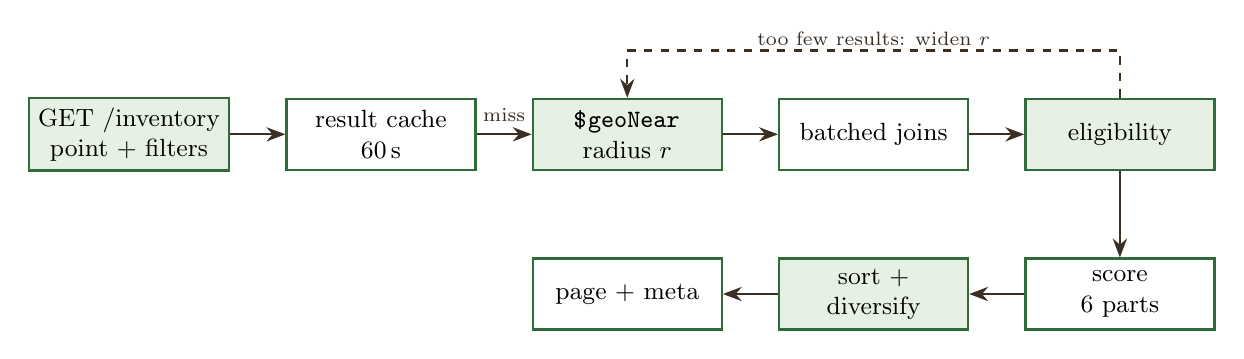
\begin{tikzpicture}[node distance=6mm and 7mm, every node/.style={font=\small}]
  \node[box, minimum width=24mm] (q) {GET /inventory\\point + filters};
  \node[box, right=of q, fill=white, minimum width=24mm] (c) {result cache\\60\,s};
  \node[box, right=of c, minimum width=24mm] (g) {\texttt{\$geoNear}\\radius $r$};
  \node[box, right=of g, fill=white, minimum width=24mm] (j) {batched joins};
  \node[box, right=of j, minimum width=24mm] (e) {eligibility};
  \node[box, below=11mm of e, fill=white, minimum width=24mm] (sc) {score\\6 parts};
  \node[box, left=of sc, minimum width=24mm] (dv) {sort +\\diversify};
  \node[box, left=of dv, fill=white, minimum width=24mm] (pg) {page + meta};
  \draw[arr] (q) -- (c); \draw[arr] (c) -- node[lbl,above=1mm]{miss} (g); \draw[arr] (g) -- (j); \draw[arr] (j) -- (e);
  \draw[arr] (e) -- (sc); \draw[arr] (sc) -- (dv); \draw[arr] (dv) -- (pg);
  \draw[arr, dashed] (e.north) -- ++(0,6mm) -| node[lbl,pos=0.25,above]{too few results: widen $r$} (g.north);
\end{tikzpicture}
\caption{Discovery pipeline (detailed in Section~\ref{sec:algo}): one indexed geo query, then three batched reads instead of thousands of per-document lookups.}
\end{figure}

\subsubsection*{Checkout: placing an order}

\begin{figure}[H]\centering
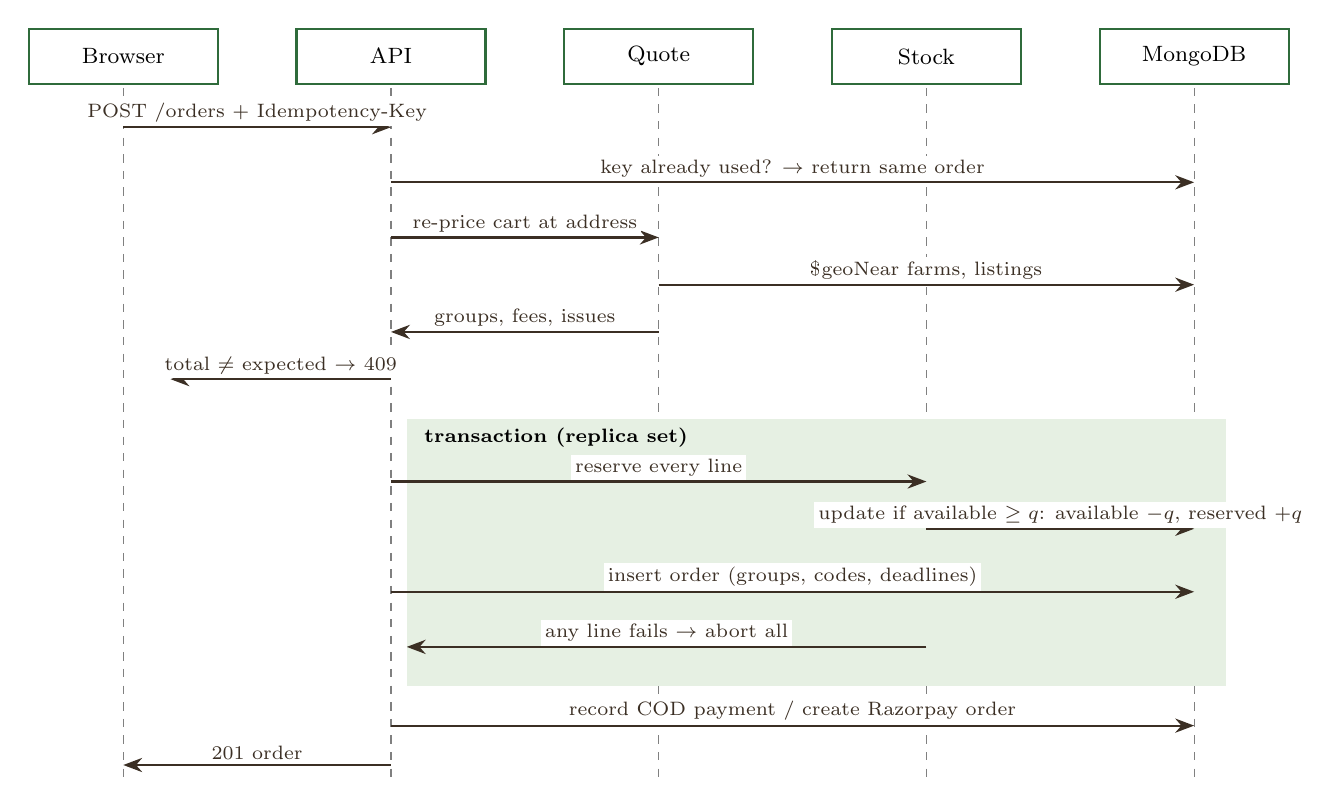
\begin{tikzpicture}[x=1mm, y=1mm, font=\footnotesize]
  \foreach \x/\n in {0/Browser, 34/API, 68/Quote, 102/Stock, 136/MongoDB}{
    \node[sbox, minimum width=24mm] (h\x) at (\x,0) {\n};
    \draw[gray, dashed] (\x,-4) -- (\x,-92);
  }
  \newcommand{\msg}[4]{\draw[arr] (#1,#3) -- node[lbl,above]{#4} (#2,#3);}
  \msg{0}{34}{-9}{POST /orders + Idempotency-Key}
  \msg{34}{136}{-16}{key already used? $\to$ return same order}
  \msg{34}{68}{-23}{re-price cart at address}
  \msg{68}{136}{-29}{\$geoNear farms, listings}
  \msg{68}{34}{-35}{groups, fees, issues}
  \draw[arr] (34,-41) -- node[lbl,above]{total $\ne$ expected $\to$ 409} (6,-41);
  \fill[leafl] (36,-46) rectangle (140,-80);
  \node[font=\scriptsize\bfseries, anchor=north west] at (37,-46) {transaction (replica set)};
  \msg{34}{102}{-54}{reserve every line}
  \msg{102}{136}{-60}{update if available $\ge q$: available $-q$, reserved $+q$}
  \msg{34}{136}{-68}{insert order (groups, codes, deadlines)}
  \draw[arr] (102,-75) -- node[lbl,above]{any line fails $\to$ abort all} (36,-75);
  \msg{34}{136}{-85}{record COD payment / create Razorpay order}
  \draw[arr] (34,-90) -- node[lbl,above]{201 order} (0,-90);
\end{tikzpicture}
\caption{Placing an order. Re-pricing on the server, idempotency and an all-or-nothing reservation guarantee that a double tap creates one order and that stock is never oversold.}
\label{fig:checkout}
\end{figure}

\subsubsection*{Delivery by a partner}

\begin{figure}[H]\centering
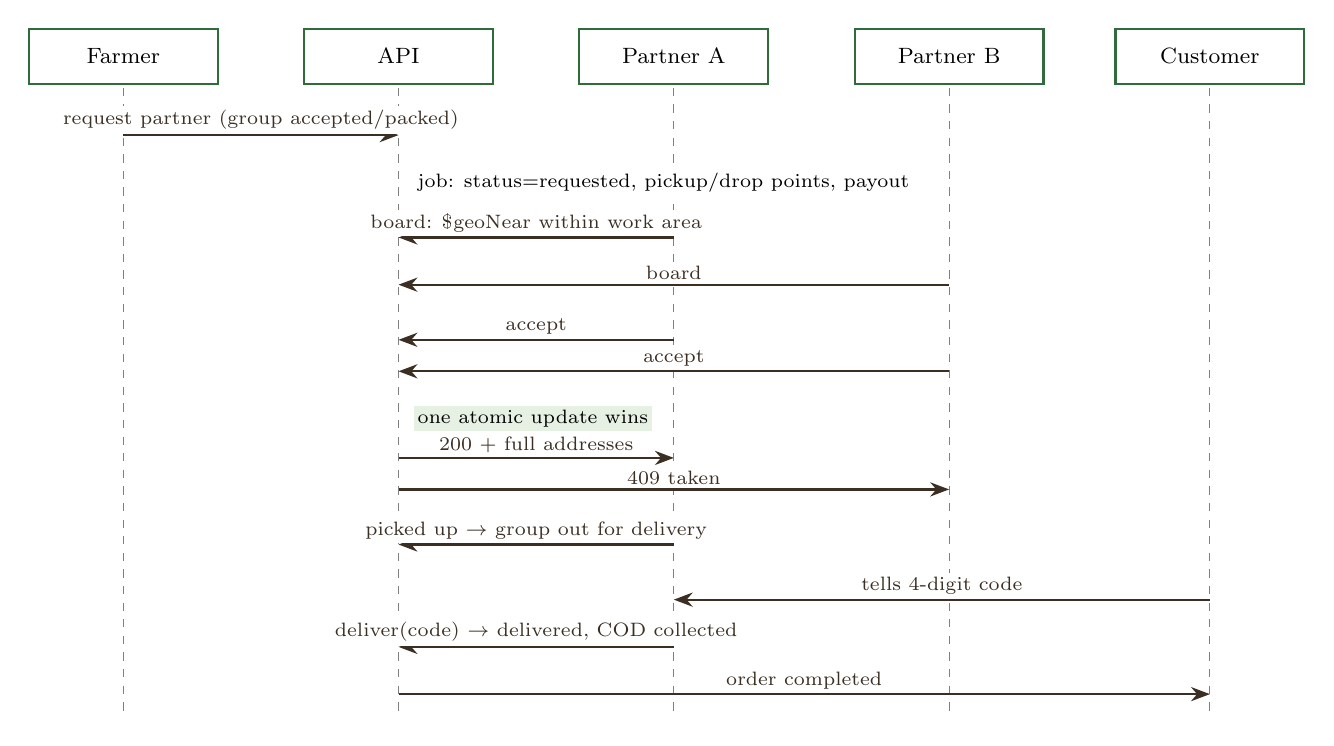
\begin{tikzpicture}[x=0.92mm, y=1mm, font=\footnotesize]
  \foreach \x/\n in {0/Farmer, 38/API, 76/Partner A, 114/Partner B, 150/Customer}{
    \node[sbox, minimum width=24mm] at (\x,0) {\n};
    \draw[gray, dashed] (\x,-4) -- (\x,-84);
  }
  \newcommand{\msg}[4]{\draw[arr] (#1,#3) -- node[lbl,above]{#4} (#2,#3);}
  \msg{0}{38}{-10}{request partner (group accepted/packed)}
  \node[lbl, anchor=west] at (40,-16) {job: status=requested, pickup/drop points, payout};
  \msg{76}{38}{-23}{board: \$geoNear within work area}
  \msg{114}{38}{-29}{board}
  \msg{76}{38}{-36}{accept}
  \msg{114}{38}{-40}{accept}
  \node[lbl, anchor=west, fill=leafl] at (40,-46) {one atomic update wins};
  \msg{38}{76}{-51}{200 + full addresses}
  \msg{38}{114}{-55}{409 taken}
  \msg{76}{38}{-62}{picked up $\to$ group out for delivery}
  \msg{150}{76}{-69}{tells 4-digit code}
  \msg{76}{38}{-75}{deliver(code) $\to$ delivered, COD collected}
  \msg{38}{150}{-81}{order completed}
\end{tikzpicture}
\caption{Delivery job life cycle. The job board shows only areas and pay; phone numbers and exact addresses are revealed to the winning partner only.}
\end{figure}

\subsubsection*{Authentication and session renewal}

\begin{figure}[H]\centering
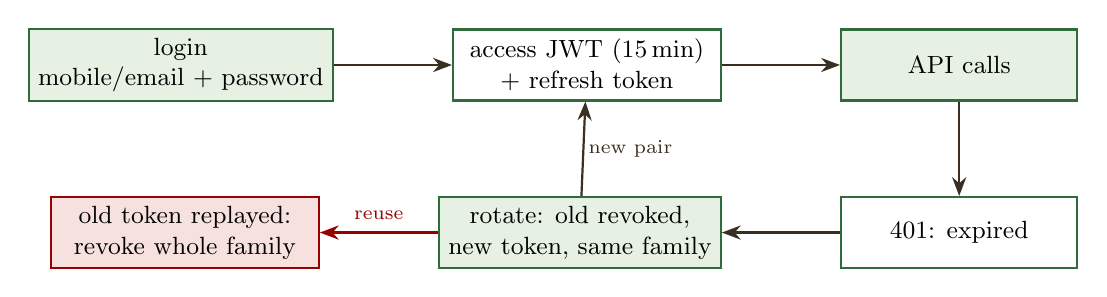
\begin{tikzpicture}[node distance=8mm and 15mm]
  \node[box, minimum width=34mm] (login) {login\\mobile/email + password};
  \node[box, right=of login, fill=white, minimum width=34mm] (pair) {access JWT (15\,min)\\+ refresh token};
  \node[box, right=of pair, minimum width=30mm] (use) {API calls};
  \node[box, below=12mm of use, fill=white, minimum width=30mm] (exp) {401: expired};
  \node[box, left=of exp, minimum width=34mm] (rot) {rotate: old revoked,\\new token, same family};
  \node[bad, left=of rot, minimum width=34mm] (reuse) {old token replayed:\\revoke whole family};
  \draw[arr] (login) -- (pair); \draw[arr] (pair) -- (use); \draw[arr] (use) -- (exp);
  \draw[arr] (exp) -- (rot);
  \draw[arr] (rot) -- node[lbl,right]{new pair} (pair);
  \draw[arr, red!60!black] (rot) -- node[lbl,above=1mm]{reuse} (reuse);
\end{tikzpicture}
\caption{Short access tokens with rotating refresh tokens. A stolen refresh token is detected the moment either party uses an old one.}
\end{figure}

\subsection{Order state machine}

\begin{figure}[H]\centering
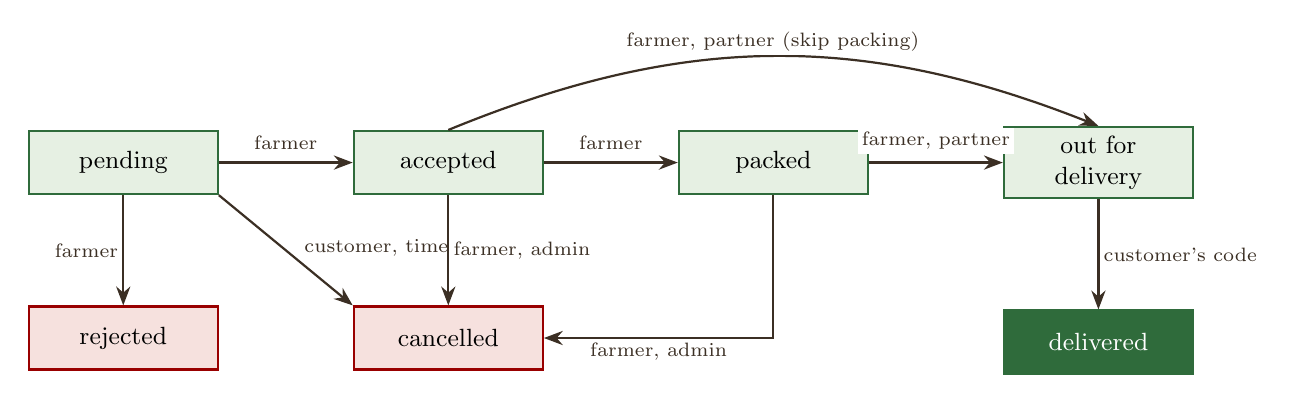
\begin{tikzpicture}[node distance=12mm and 17mm]
  \node[state] (p) {pending};
  \node[state, right=of p] (a) {accepted};
  \node[state, right=of a] (k) {packed};
  \node[state, right=of k] (o) {out for\\delivery};
  \node[state, below=14mm of o, fill=leaf, text=white] (d) {delivered};
  \node[bad, below=14mm of p] (r) {rejected};
  \node[bad, below=14mm of a] (c) {cancelled};
  \draw[arr] (p) -- node[lbl,above=1mm]{farmer} (a);
  \draw[arr] (a) -- node[lbl,above=1mm]{farmer} (k);
  \draw[arr] (k) -- node[lbl,above=1mm]{farmer, partner} (o);
  \draw[arr] (a.north) to[bend left=22] node[lbl,above]{farmer, partner (skip packing)} (o.north);
  \draw[arr] (o) -- node[lbl,right]{customer's code} (d);
  \draw[arr] (p) -- node[lbl,left]{farmer} (r);
  \draw[arr] (p.south east) -- node[lbl,pos=0.6,above right]{customer, timeout} (c.north west);
  \draw[arr] (a) -- node[lbl,right]{farmer, admin} (c);
  \draw[arr] (k.south) |- node[lbl,pos=0.75,below]{farmer, admin} (c.east);
\end{tikzpicture}
\caption{Life cycle of one farm's part of an order. Every transition is one conditional update (\emph{only if the current status is one of the allowed sources}), so concurrent clicks, the deadline job and an admin can never both apply. Stock is released on rejected or cancelled and consumed on delivered.}
\label{fig:fsm}
\end{figure}

\noindent The order's own status (\emph{placed, in progress, completed, cancelled}) and its payment status are \textbf{derived} from its groups after every transition, never edited directly. For example, a cash-on-delivery order is \emph{paid} once every live group is delivered, and a paid online order with a cancelled part owes exactly that part's total as a refund.

\subsection{Consistency and concurrency}

\begin{itemize}
  \item \textbf{Conditional updates as the unit of correctness.} Every contended write is a single document update with its precondition in the filter. Examples: stock (\texttt{quantityAvailable $\ge q$}), order transitions (\texttt{status $\in$ allowed}), job claims (\texttt{status=requested, partner=null}), refund records (document version). The database serialises them; no application locks are needed.
  \item \textbf{Transactions where several documents must change together.} Reserving stock for every line and inserting the order happen in one multi-document transaction on the replica set. On a standalone server (development) the same code falls back to compensation: reservations already made are released if a later step fails.
  \item \textbf{Idempotency.} The checkout's unique \texttt{(customer, idempotencyKey)} index makes retries and double taps return the original order.
  \item \textbf{Safety nets.} An hourly job recomputes reserved stock from open orders and reports any drift. A reconciliation job asks Razorpay about payments whose callback never arrived before an unpaid order is cancelled.
\end{itemize}

\subsection{Security architecture}

\begin{table}[H]\centering\small
\begin{tabularx}{\linewidth}{@{}p{3.3cm}L@{}}
\toprule
\textbf{Threat} & \textbf{Control} \\
\midrule
Stolen session & 15-minute access tokens; refresh tokens stored only as SHA-256 hashes, rotated on every use, revoked as a family on reuse; httpOnly cookies scoped to \texttt{/api/auth}; logout everywhere; suspension ends all sessions. \\
Password guessing & bcrypt hashes; 20 attempts per 15 minutes per IP on credential endpoints; identical errors for unknown account and wrong password. \\
Account enumeration & Password reset answers identically for unknown accounts and sends mail in the background so timing reveals nothing. \\
Fake delivery & 4-digit handover code known only to the customer; wrong attempts counted atomically and the code locks after 5, so guessing has at most a $5/10^4$ chance. The customer can issue a new code. \\
Privilege abuse & Role checks on every route; partners see contact details only for jobs they hold; farmers never see handover codes; every admin action is written to an append-only audit trail with a mandatory reason for negative decisions. \\
Injection and bad input & Zod validation of every body, query and parameter; regular expressions built only from escaped input; images only from approved hosts; uploads restricted by type. \\
Network exposure & API and database bound to localhost; database authentication with separate admin and application users; one public port. \\
\bottomrule
\end{tabularx}
\caption{Threats and controls.}
\end{table}

\subsection{Caching strategy}

\begin{table}[H]\centering\small
\begin{tabularx}{\linewidth}{@{}p{3cm}p{3.6cm}L@{}}
\toprule
\textbf{Layer} & \textbf{What} & \textbf{Freshness rule} \\
\midrule
Browser (HTTP) & public lists & \texttt{no-cache} + ETag: always revalidated, \texttt{304} when unchanged. \\
Client query cache & every screen's data & 15\,s fresh; refetch on focus; invalidated by area after writes; polling for live queues. \\
API result cache & discovery results & 60\,s; key rounds coordinates to $\approx$110\,m; cleared on any farm, listing, stock or verification change. In-memory, or Redis when several API processes run. \\
API catalogue cache & product definitions & short TTL; the catalogue changes rarely. \\
Geocoding & place search & cached and throttled to respect OpenStreetMap's usage policy. \\
\bottomrule
\end{tabularx}
\caption{Caching layers and how each stays correct.}
\end{table}

\subsection{Background jobs}

\begin{table}[H]\centering\small
\begin{tabular}{@{}llp{8cm}@{}}
\toprule
\textbf{Job} & \textbf{Every} & \textbf{Purpose} \\
\midrule
expire-unpaid-orders & 1 min & Cancel online orders not paid within 15 min and release their stock, after asking Razorpay first. \\
expire-unaccepted-orders & 5 min & Cancel farm parts not accepted within 24 h so stock is not held forever. \\
reconcile-payments & 5 min & Find payments captured at Razorpay whose callback never arrived. \\
check-reserved-stock & 1 h & Recompute reserved stock from open orders and report drift. \\
\bottomrule
\end{tabular}
\caption{Scheduled jobs (in-process at launch; a job queue is the next step at scale).}
\end{table}

\subsection{Scaling path}

\begin{enumerate}
  \item \textbf{Several API processes} (one per core) behind the web proxy or a load balancer, with Redis for the shared result cache and rate limits. The API is stateless, so this needs no code change.
  \item \textbf{Native password hashing} (bcrypt on the libuv thread pool) so bursts of logins do not block other requests (Section~\ref{sec:eval}).
  \item \textbf{A job queue} (e.g. BullMQ) so scheduled work runs once across many processes.
  \item \textbf{Push instead of polling} (server-sent events) for the job board and order queues, which are the dominant source of traffic.
  \item \textbf{Shard by city.} Farms, listings and orders all carry a city key and almost all queries are local, so cities partition naturally.
\end{enumerate}

%======================================================================
\section{Algorithms}\label{sec:algo}
%======================================================================

\begin{table}[H]\centering\small
\begin{tabularx}{\linewidth}{@{}p{3.6cm}p{3.2cm}p{2.2cm}L@{}}
\toprule
\textbf{Algorithm} & \textbf{Used in} & \textbf{Cost} & \textbf{Why here} \\
\midrule
2dsphere index + \texttt{\$geoNear} & discovery, job board, checkout distances & $O(\log n + k)$ & exact spherical distances, sorted, index-backed \\
Adaptive radius widening & discovery & $\le 3$ queries & dense areas stay local; sparse areas still get results \\
Hybrid weighted scoring & product and farm ranking & $O(k)$ & transparent, tunable, works with no history \\
Bayesian average rating & ranking & $O(1)$ & one 5-star review must not beat 200 good ones \\
Grouped min--max price & ranking & $O(k)$ & only like-for-like items compared \\
Greedy diversity re-rank & recommended order & $O(k\cdot m)$ & one big farm cannot fill the first page \\
Conditional atomic update & stock, transitions, claims & $O(1)$ & correctness without locks \\
Finite-state machine & order groups & $O(1)$ & illegal transitions impossible \\
Token rotation + reuse detection & sessions & $O(1)$ & detects stolen refresh tokens \\
Attempt-counted one-time code & handover & $O(1)$ & brute force bounded at 0.05\% \\
\bottomrule
\end{tabularx}
\caption{Algorithms at a glance ($n$ = indexed documents, $k$ = candidates near the customer, $m$ = page size).}
\end{table}

\subsection{Geo-spatial retrieval}

\paragraph{Problem.} Given a customer at point $P$, find every listing whose farm is within the search radius $r$ \emph{and} whose farm delivers to $P$ (its own radius $R_f$), in distance order.

\paragraph{Approach.} Points are stored as GeoJSON with a \textbf{2dsphere} index. MongoDB's \texttt{\$geoNear} stage walks the index outward from $P$ (an S2 cell covering of the sphere), returning candidates already sorted by great-circle distance
\[
  d(P,Q) = 2R\arcsin\sqrt{\sin^2\tfrac{\Delta\varphi}{2} + \cos\varphi_P\cos\varphi_Q\sin^2\tfrac{\Delta\lambda}{2}}
\]
together with the distance itself. The stage's filter applies eligibility that can be expressed on the listing (active, in stock, not expired). A second, per-farm condition $d(P,f) \le R_f$ is applied after joining farms, because every farm has its own radius.

\paragraph{Why this and not alternatives.}
\begin{itemize}
  \item \emph{Computing the haversine distance in application code} for every listing is $O(n)$ per request and does not scale beyond a few thousand listings.
  \item \emph{Geohash or H3 grids} need neighbour-cell expansion and still require exact distance for ordering and radius checks; the 2dsphere index already provides both.
  \item \emph{A separate search engine} adds an operational component for a capability the primary database already has.
\end{itemize}

\paragraph{Batched joins.} Candidates reference farms, farmers and catalogue products. Instead of a \texttt{\$lookup} per candidate, the service collects the distinct ids and loads each collection with one \texttt{\$in} query (the catalogue comes from memory). On a city-sized benchmark this replaced about 3{,}000 per-document lookups per request with three reads.

\subsection{Adaptive radius widening}

\begin{algorithm}[H]
\caption{Search radius selection}
\begin{pseudo}
  \item \kw{input:} point $P$; steps $S = [8, 15, 25]$\,km; minimum results $N$ (8 products or 4 farms)
  \item \kw{for} $r \in S$ \kw{do}
  \item \ind $C \gets$ eligible candidates within $r$
  \item \ind \kw{if} $|C| \ge N$ \kw{then return} $(C, r)$
  \item \kw{return} $(C, \text{last } r)$ \hfill \emph{the response says the search was widened}
\end{pseudo}
\end{algorithm}

\noindent \textbf{Why.} In a dense neighbourhood customers should see their closest farms, not farms 20\,km away that happen to be cheaper. On the city's edge the same fixed radius would return nothing. Widening only when needed gives both behaviours, and the user interface tells the customer that farms further away are being shown. An explicit radius chosen by the user is respected exactly.

\subsection{Hybrid weighted scoring}

Each candidate gets six component scores in $[0,1]$, combined by a weighted mean:
\[
  \text{score} = \frac{\sum_i w_i\,s_i}{\sum_i w_i}
\]
with weights proximity $0.30$, freshness $0.20$, stock $0.10$, rating $0.15$, price $0.15$ and organic $0.10$ (configuration, tunable without code changes).

\begin{table}[H]\centering\small
\begin{tabularx}{\linewidth}{@{}p{2.2cm}p{6.3cm}L@{}}
\toprule
\textbf{Part} & \textbf{Formula} & \textbf{Reasoning} \\
\midrule
Proximity & $1 - d/r$ & closer is fresher and cheaper to deliver; relative to the radius actually searched \\
Freshness (fresh) & $1 - \text{age}/\text{shelfLife}$ & a 2-day-old tomato (7-day shelf life) beats a 5-day-old one \\
Freshness (dry) & $(\text{expiry} - \text{now}) / (\text{expiry} - \text{processed})$ & remaining shelf life of packaged goods \\
Stock & $\min\!\big(1, \frac{\text{available}}{10 \cdot \text{minOrder}}\big)$ & prefers listings that can serve many orders; saturates \\
Rating & $\big(\frac{\bar r\,n + 3.5\cdot 5}{n + 5} - 1\big)/4$ & Bayesian average: few reviews are pulled toward the prior 3.5 \\
Price & $\frac{p_{\max} - p}{p_{\max} - p_{\min}}$ within (product, unit, pack size) & compares only like-for-like offers \\
Organic & 1 if the certificate is verified by an admin & claims alone do not count \\
\bottomrule
\end{tabularx}
\caption{Score components.}
\end{table}

\paragraph{Why a weighted model instead of machine learning.} At launch there is no interaction history to learn from (the cold-start problem). A transparent weighted model:
\begin{itemize}
  \item can be explained to farmers (``you rank lower because your tomatoes are 5 days old'');
  \item can be tuned by business priority (weights are configuration);
  \item works from the first day.
\end{itemize}
Each part is returned with every result, so the ranking can be audited, as the independent checker in Section~\ref{sec:eval} does. Once orders accumulate, the same parts become features for a learning-to-rank model behind the same interface.

\paragraph{Bayesian rating, example.} A farmer with one 5-star review gets $(5\cdot1+3.5\cdot5)/6 = 3.75$; a farmer with 200 reviews averaging 4.7 gets $(4.7\cdot200+17.5)/205 \approx 4.67$. The established farmer correctly ranks higher.

\subsection{Greedy diversity re-ranking}

Sorting purely by score lets one large farm with ten good listings fill the whole first page. The recommended order applies a greedy re-rank in the spirit of maximal marginal relevance:

\begin{algorithm}[H]
\caption{Farm-diversity re-rank (decay $\delta = 0.85$)}
\begin{pseudo}
  \item \kw{input:} items sorted by score; page size $m$
  \item $\text{picked}[f] \gets 0$ for every farm $f$; $\text{out} \gets [\,]$
  \item \kw{while} $|\text{out}| < m$ \kw{and} items remain \kw{do}
  \item \ind choose the item $x$ maximising $\text{score}(x)\cdot\delta^{\,\text{picked}[\text{farm}(x)]}$
  \item \ind append $x$ to out; $\text{picked}[\text{farm}(x)] \gets \text{picked}[\text{farm}(x)] + 1$
  \item \kw{return} out followed by the remaining items in score order
\end{pseudo}
\end{algorithm}

\noindent \textbf{Why.} Customers benefit from comparing farms, and small farms get visibility. The penalty is soft: an outstanding second item from the same farm still appears early. Cost is $O(k\cdot m)$ for the page only, rather than $O(k^2)$ for the whole list. Explicit sorts (distance, price, freshness) keep their exact order.

\subsection{Sellability rule}

One predicate decides whether a listing can be sold right now, and it is shared by search, farm lists, product pages, farmer profiles and checkout:
\[
\text{sellable} \iff \text{active} \wedge \text{available} \ge \text{minOrder} \wedge
\begin{cases}
\text{now} - \text{harvest} \le \text{shelfLife} & \text{fresh}\\
\text{expiry} > \text{now} & \text{dry}
\end{cases}
\]
It is compiled once into a database filter (one clause per catalogue product for the fresh case) so the geo query applies it inside the index scan. \textbf{Why:} the verification in Section~\ref{sec:eval} found that, before this rule existed, expired goods were offered and listings with less stock than one minimum order were shown but could never be ordered. A single shared definition makes ``shown'' and ``orderable'' the same set by construction.

\subsection{Atomic stock reservation}

\begin{algorithm}[H]
\caption{Reserve stock for an order (inside one transaction)}
\begin{pseudo}
  \item \kw{for each} line $(\ell, q)$ \kw{do}
  \item \ind \texttt{updateOne(\{\_id: $\ell$, available: \{\$gte: $q$\}\}, \{\$inc: \{available: $-q$, reserved: $+q$\}\})}
  \item \ind \kw{if} no document matched \kw{then} abort the transaction; report ``only $x$ left''
  \item insert the order; commit
\end{pseudo}
\end{algorithm}

\noindent \textbf{Why.} The availability check and the decrement are one atomic operation, so two buyers racing for the last units cannot both succeed: the second update simply matches no document. Locks or ``read then write'' would either serialise all checkouts or allow overselling. Delivered groups convert reserved into sold; rejected and cancelled groups release it. A test races six buyers for three units and asserts exactly three units are sold.

\subsection{Delivery job matching}

Open jobs carry the farm's point. A partner's board is a \texttt{\$geoNear} from the partner's base within their work area, filtered to \texttt{status = requested}, nearest pickup first. Claiming is one conditional update:
\begin{center}\small
\texttt{findOneAndUpdate(\{\_id, status: requested, partner: null\},}\\
\texttt{\phantom{findOneAndUpdate(}\{status: assigned, partner: me\})}
\end{center}
Payout is $\max(30,\; 20 + 6 \times \text{tripKm})$ rupees.

\paragraph{Why first-wins self-selection rather than central dispatch.} Centrally optimal assignment (e.g.\ the Hungarian algorithm or vehicle-routing heuristics) pays off with large, full-time fleets and dense demand. At launch, partners are independent and part-time and know local roads. Each job is one pickup and one drop. A geo-filtered board with an atomic claim is simple, fair, explainable and correct under concurrency. A cap on simultaneous jobs (3 by default) keeps partners from hoarding work. Central batching can be added later behind the same job records.

\subsection{Session security algorithms}

\paragraph{Refresh-token rotation with reuse detection.} A refresh token is \texttt{sessionId.secret}; only $\text{SHA-256}(\text{secret})$ is stored. Each use revokes the session and issues a new one in the same \emph{family}. If a revoked token is presented again after a 30-second grace window, which allows two browser tabs to refresh at once, someone holds a copy: the whole family is revoked, logging out both the attacker and the victim, who must sign in again. The load test confirmed the mechanism: every replayed stale token was detected (43 of 43).

\paragraph{Handover code with attempt counting.} Each farm part gets a random 4-digit code shown only to the customer. Wrong attempts are counted with an atomic increment, and after 5 the code locks until the customer issues a new one. A dishonest deliverer's chance of guessing is therefore at most $5/10{,}000 = 0.05\%$, instead of certainty after about 34 minutes of trying at the API's rate limit.

\subsection{Delivery fee}
\[
\text{fee}(s, d) = \begin{cases} 0 & s \ge 300 \\ \min(60,\; 20 + 3\lceil d \rceil) & \text{otherwise} \end{cases}
\]
for farm subtotal $s$ (rupees) and distance $d$ (km), charged per farm because each farm delivers separately. The free threshold nudges customers toward larger baskets from fewer farms, which also reduces delivery trips.

%======================================================================
\section{Functionality}
%======================================================================

\subsection{Customer}

\shot{01-home}{Home page with search, categories of fresh and dry produce and the delivery location in the header.}
\shot{02-home-nearby}{``Farmers near you'': ranked farms with distance, organic verification, rating and starting prices.}
\shot{03-shop}{Shop: every listing that delivers to the customer, with search, type, distance, price and organic filters. The count states the location used.}
\shot{04-product}{Product page: price, freshness, delivery check for this address, the farmer and the farm, and the same product from other farms.}
\shot{05-farmer-profile}{Public farmer profile with story, practices, farms on a map and products in stock.}
\shot{08-cart}{Cart grouped by farm, priced live by the server, with delivery fee per farm and the free-delivery threshold.}
\shot{09-checkout}{Checkout: saved address, payment method and the server-checked order summary.}
\shot{11-order-tracking}{Order tracking: per-farm progress, the 4-digit delivery code, expected date and the delivery partner on the way.}

\subsection{Sign-in}

\begin{figure}[H]\centering
\begin{subfigure}{0.49\linewidth}\centering\fbox{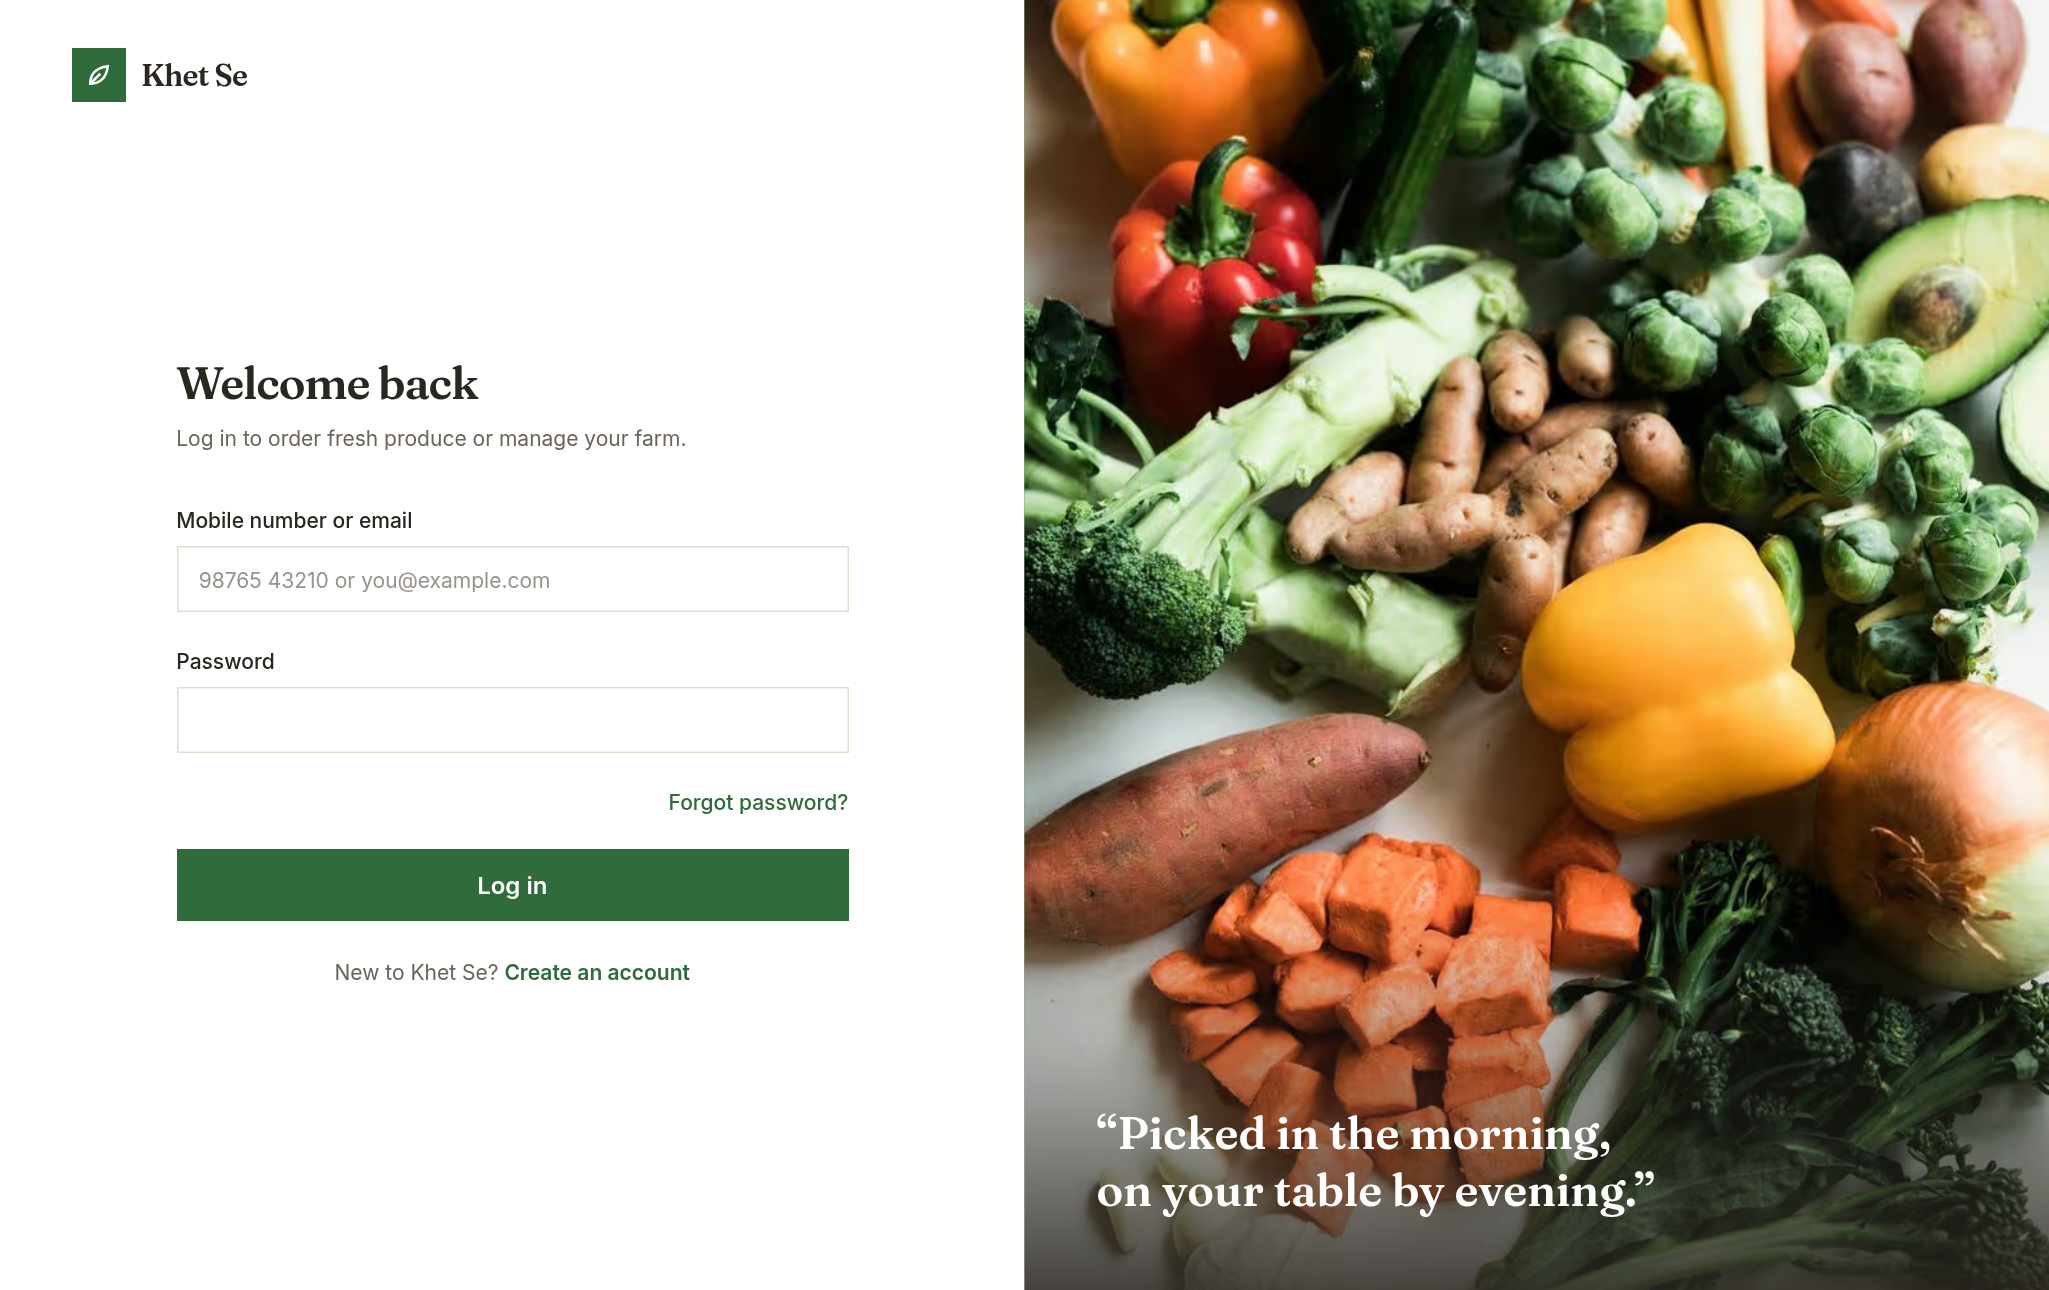
\includegraphics[width=0.96\linewidth]{06-login}}\caption{Login with mobile number or email.}\end{subfigure}\hfill
\begin{subfigure}{0.49\linewidth}\centering\fbox{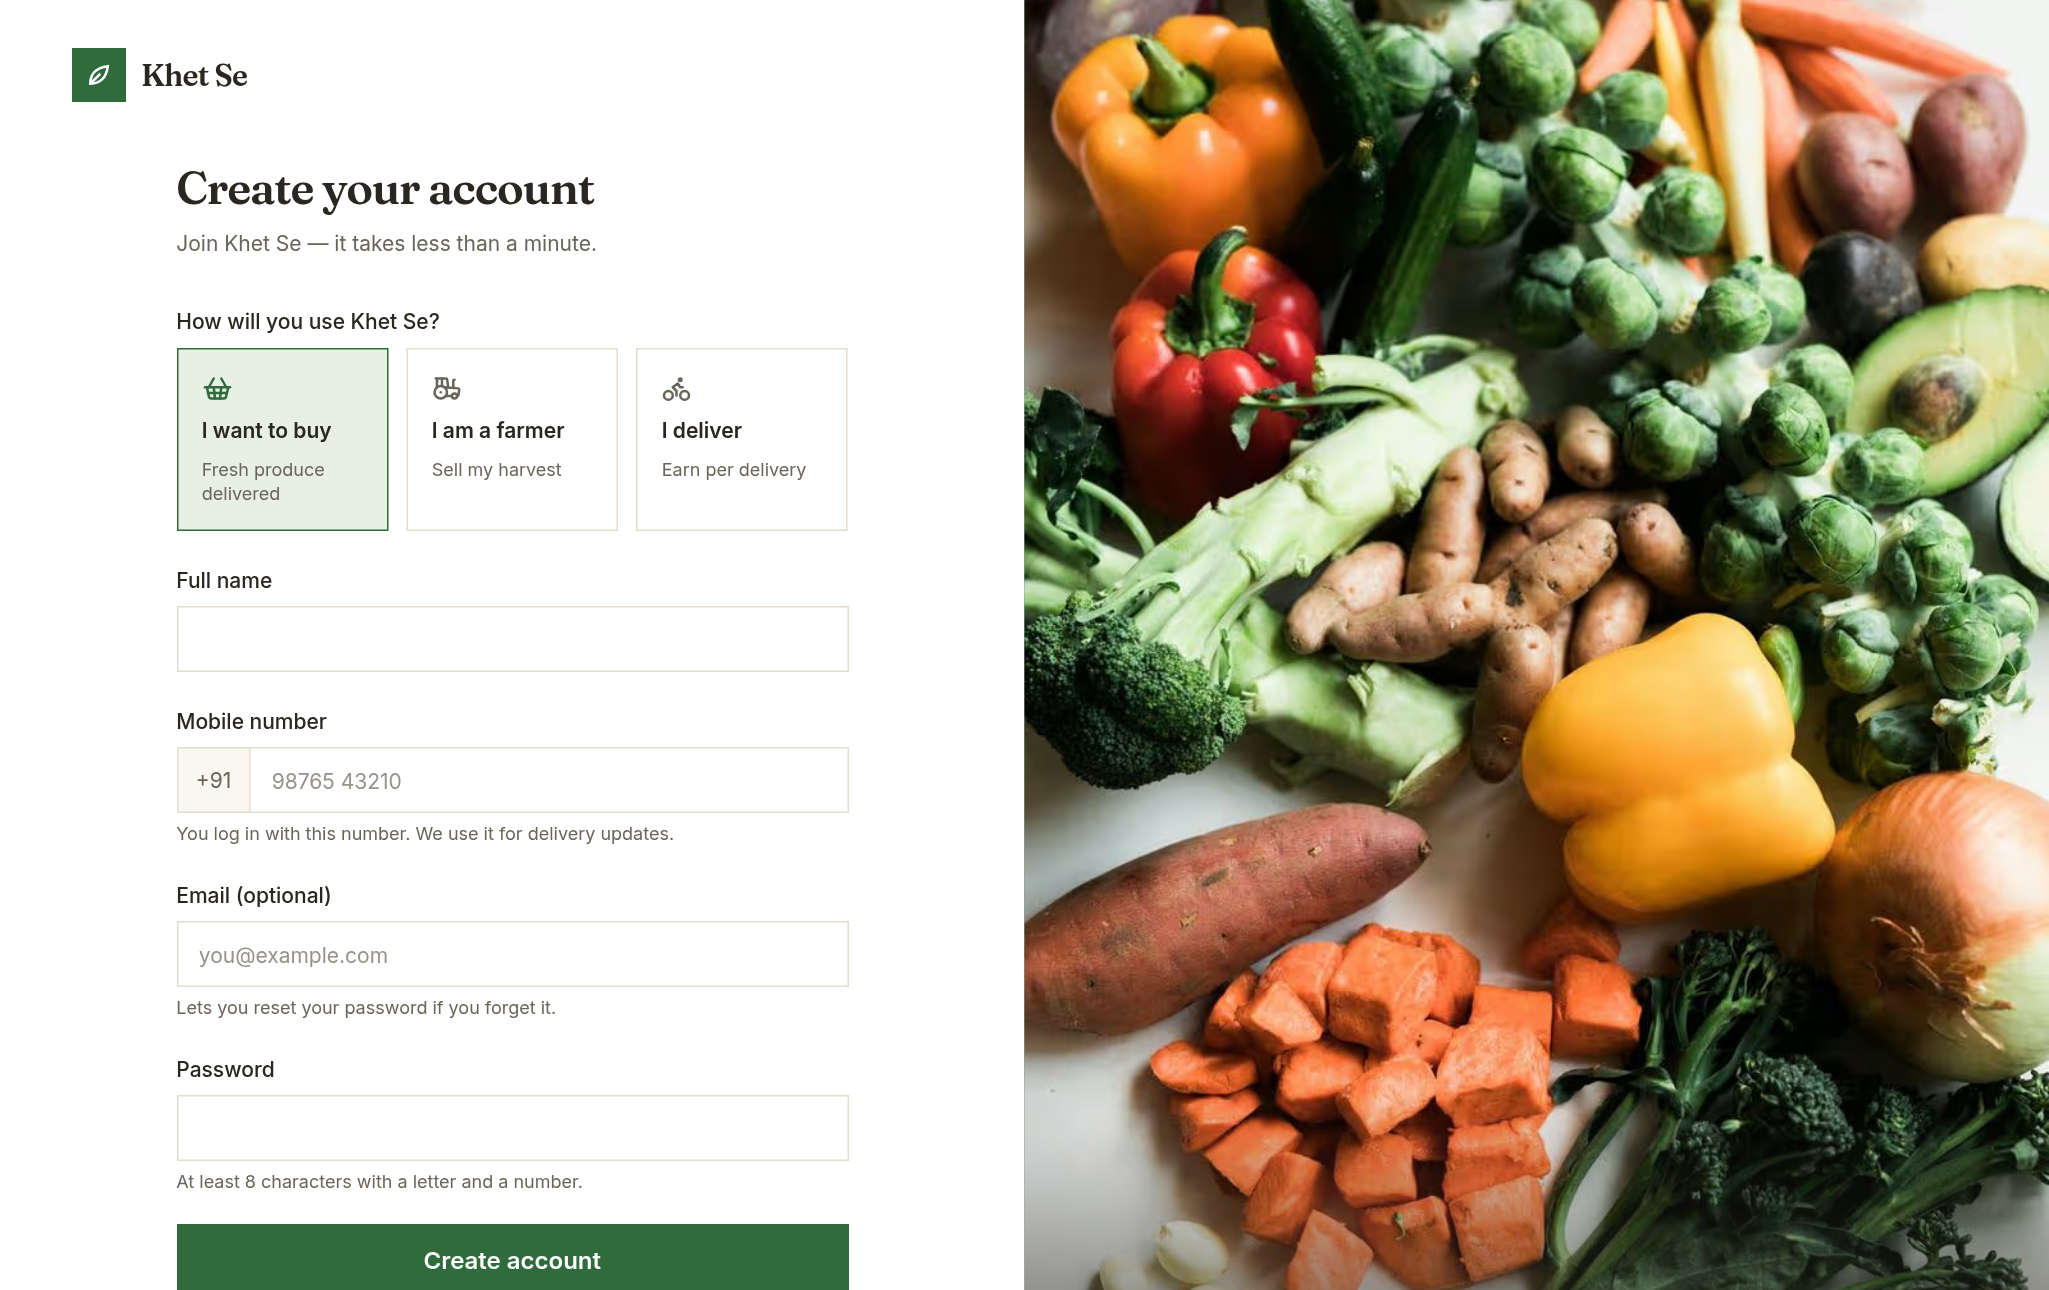
\includegraphics[width=0.96\linewidth]{07-register}}\caption{Sign-up with role choice; email is optional.}\end{subfigure}
\caption{Authentication screens.}
\end{figure}

\subsection{Farmer}

\shot{12-farmer-overview}{Farmer dashboard: set-up checklist, orders to deliver, products on sale, low and out-of-stock counts, verification status.}
\shot{13-farmer-orders}{Incoming orders with the customer's address, distance, acceptance deadline and the choice to deliver personally or request a partner.}
\shot{14-farmer-to-deliver}{Orders to deliver, showing which partner is collecting or on the way.}
\shot{15-farmer-inventory}{Inventory: stock levels, quick stock edits and status filters.}

\subsection{Delivery partner}

\shot{16-partner-overview}{Partner overview: online switch, earnings, distance, cash collected and active jobs.}
\shot{17-partner-board}{Job board: open deliveries in the work area with pay, trip length, pickup distance and cash to collect. Contact details appear only after accepting.}
\shot{18-partner-active}{Active deliveries: call and directions for pickup and drop, ``picked up'', then hand-over with the customer's code.}

\subsection{Administrator}

\shot{19-admin-overview}{Admin overview: what needs attention (farmers to verify, orders waiting, jobs without a partner, refunds owed) and business numbers.}
\shot{20-admin-verification}{Farmer verification: details, farms, certificate and decisions; rejections require a reason that the farmer sees.}
\shot{21-admin-orders}{Orders with status, payment and refund filters and search by order number, name or mobile.}
\shot{22-admin-order-detail}{Order detail for support: each farm's part, history, codes, partner and payout, payments, refunds and admin history.}
\shot{23-admin-people}{People: search and filter customers, farmers, partners and admins; open any account to suspend or reactivate.}
\shot{24-admin-audit}{Audit trail: every admin decision with who, what, when and why.}

\subsection{Phones}

\begin{figure}[H]\centering
\begin{subfigure}{0.32\linewidth}\centering\fbox{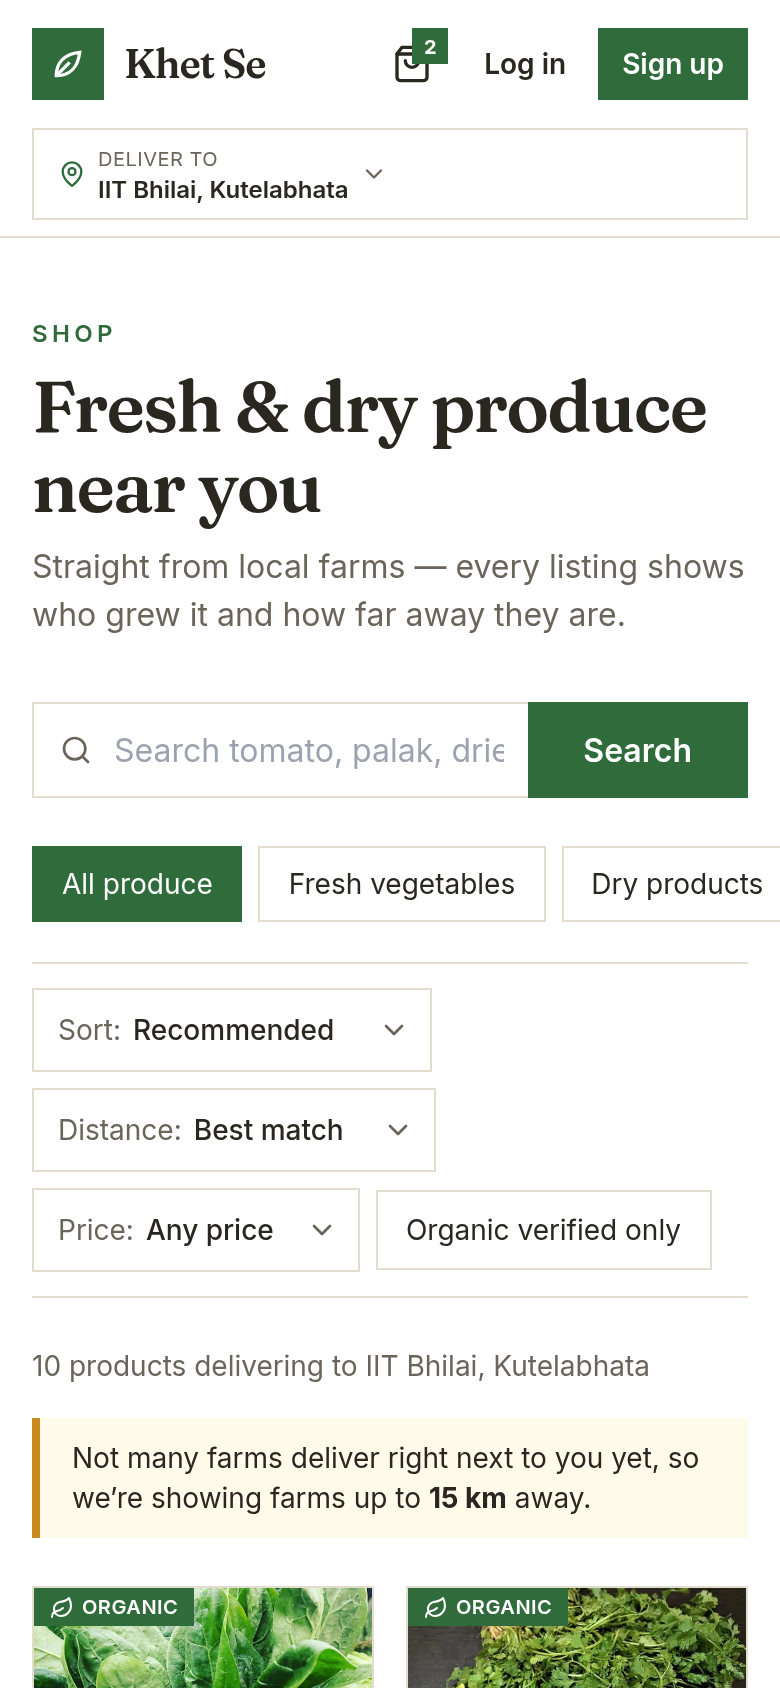
\includegraphics[width=0.95\linewidth]{25-mobile-shop}}\caption{Shop.}\end{subfigure}\hspace{8mm}
\begin{subfigure}{0.32\linewidth}\centering\fbox{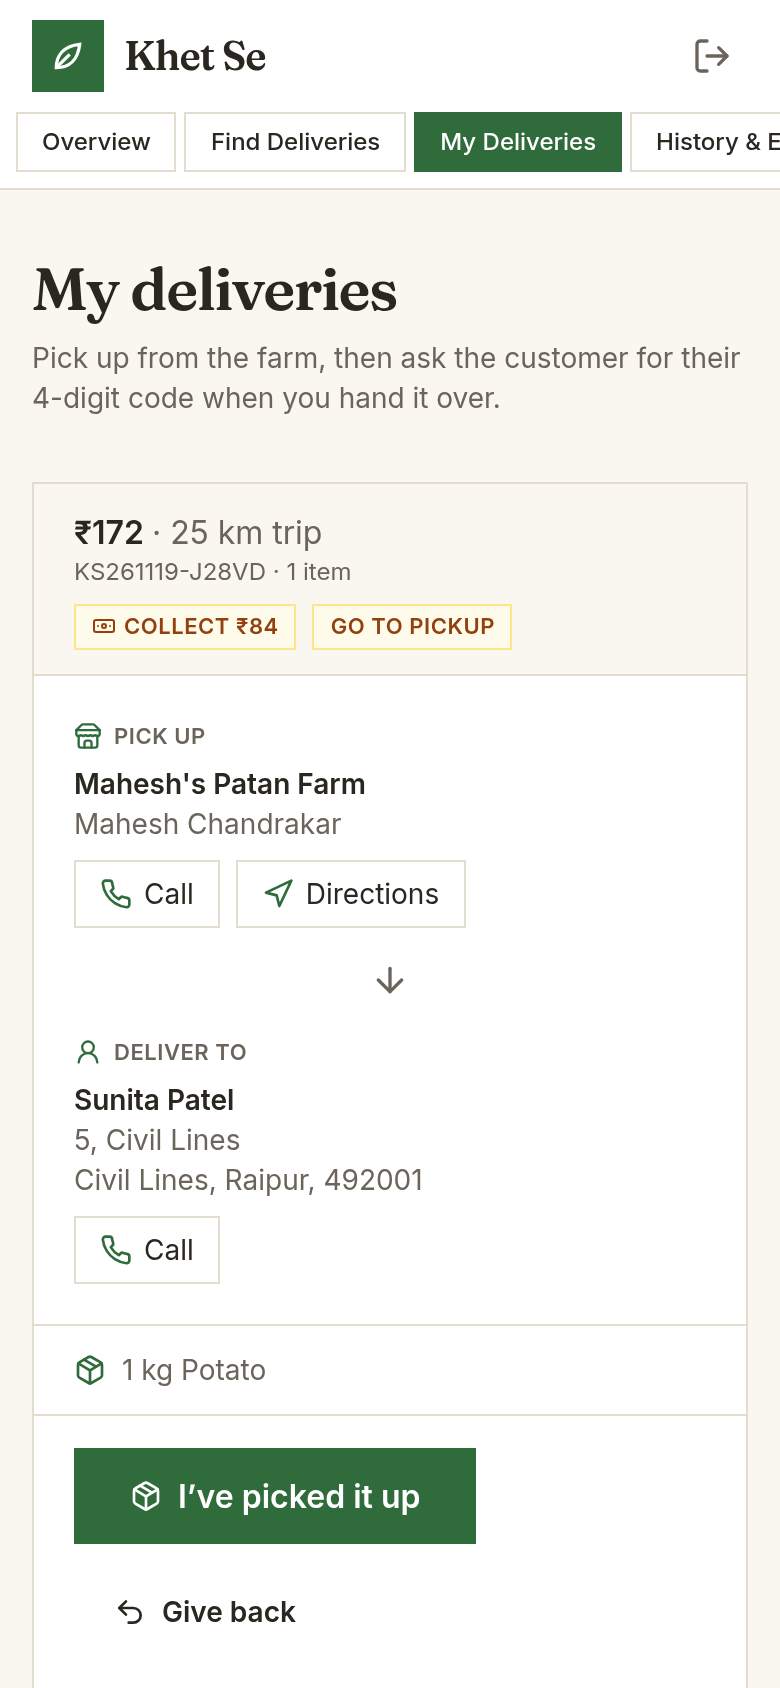
\includegraphics[width=0.95\linewidth]{26-mobile-partner}}\caption{Partner's active deliveries.}\end{subfigure}
\caption{Mobile layouts: the primary devices for farmers and partners.}
\end{figure}

%======================================================================
\section{Verification and Evaluation}\label{sec:eval}
%======================================================================

\subsection{Test strategy}

\begin{table}[H]\centering\small
\begin{tabularx}{\linewidth}{@{}p{3.6cm}L r@{}}
\toprule
\textbf{Level} & \textbf{What it proves} & \textbf{Count} \\
\midrule
Unit & scoring formulas, state rules, cache invalidation map, phone parsing & 20+ \\
API integration & real HTTP against an in-memory MongoDB replica set (real transactions): auth, sessions, inventory, discovery, checkout races, payments, delivery, admin & 138 \\
Role journeys & one end-to-end story per actor through the API, plus role isolation & 6 \\
Algorithm oracle & 3{,}469 independent checks on a real-place test bed & 1 suite \\
Load model & three personas at launch peak, stress and a capacity ramp & 3 profiles \\
\bottomrule
\end{tabularx}
\caption{Verification layers. The API suite also passes on the deployment server against MongoDB 7.}
\end{table}

\subsection{Independent algorithm verification}

A test bed of 21 farms and 27 customers was placed at real Durg--Bhilai locations, with coordinates taken from OpenStreetMap. Each farm exercises one rule:
\begin{itemize}
  \item three competing tomato farms side by side;
  \item a 3\,km farm with customers at 2.8, 2.95, 3.03, 3.05 and 3.2\,km;
  \item far farms that appear only when the search widens;
  \item a ten-listing farm for diversity;
  \item expired, stale, sold-out, paused, delivery-off, inactive and suspended cases that must never be shown.
\end{itemize}
A checker recomputes, from the raw database and with its own distance maths and formula implementations, what the API must return for each customer, and compares that with the running API.

\begin{table}[H]\centering\small
\begin{tabularx}{\linewidth}{@{}Lp{6cm}@{}}
\toprule
\textbf{Defect found} & \textbf{Fix} \\
\midrule
Expired dry goods and produce past shelf life were offered and orderable. & Shared sellable rule in every path. \\
A listing with less stock than one minimum order was shown but could never be ordered. & Search requires stock $\ge$ minimum order. \\
Checkout rounded the distance before comparing it with the delivery radius, so between 3.00 and 3.05\,km it accepted what search hid. & Exact comparison; rounding only for display and fees. \\
Price scores skewed by the expired items. & Resolved by the first fix. \\
\bottomrule
\end{tabularx}
\caption{Defects found by the algorithm checker.}
\end{table}

\begin{table}[H]\centering\small
\begin{tabular}{@{}lr@{}}
\toprule
\textbf{Check} & \textbf{Passed} \\
\midrule
Shown $\Leftrightarrow$ orderable (search and checkout agree) & 734 \\
Delivery fee rule & 563 \\
Distances within 50\,m (listings / farms) & 525 / 163 \\
Score parts / weighted totals & 525 / 525 \\
Stored listing location = farm location & 124 \\
Eligibility, radius widening, five sort orders, diversity, filters & 27 each \\
\midrule
\textbf{Total} & \textbf{3{,}469 (0 failures)} \\
\bottomrule
\end{tabular}
\caption{Algorithm verification after the fixes.}
\end{table}

\subsection{Workload model and performance}

The workload generator simulates the three populations together against a production build:
\begin{itemize}
  \item \textbf{Customers:} arrivals follow a Poisson process at 18.7 sessions per minute times a multiplier. The mix is 62.5\% browse, 10\% abandoned cart, 12.5\% buy and 15\% track.
  \item \textbf{Farmers:} 200 farmers check their queues every 60--120\,s, then accept, pack, deliver or request a partner.
  \item \textbf{Partners:} 60 partners refresh the board every 15--25\,s, then claim, pick up and hand over.
\end{itemize}
Every simulated person has its own client IP, so the real per-IP rate limits apply, and uses real token refresh. Think and travel times are compressed; arrival rates are not, so request rates match the model.

\begin{table}[H]\centering\small
\begin{tabular}{@{}lrrrrr@{}}
\toprule
\textbf{Profile} & \textbf{req/s} & \textbf{Reads p95} & \textbf{Writes p95} & \textbf{Errors} & \textbf{API CPU} \\
\midrule
Launch peak (1$\times$, 5 min) & 13.3 & 20\,ms & 31\,ms & 0 & 12\% \\
Stress (3$\times$, 3 min) & 17.0 & 28\,ms & 33\,ms & 0 & 16\% \\
\bottomrule
\end{tabular}
\caption{Launch-peak and stress results (one API process). All service-level objectives met.}
\end{table}

\begin{figure}[H]\centering
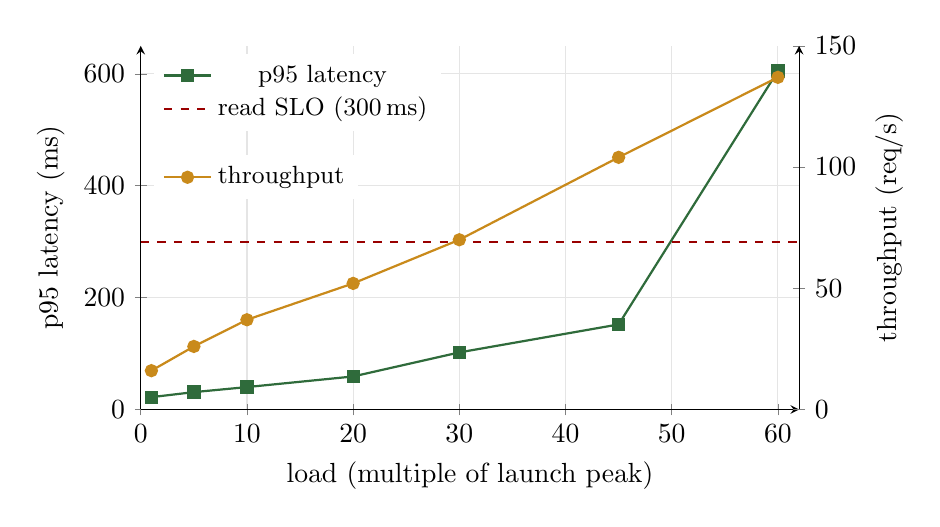
\begin{tikzpicture}
\begin{axis}[
  width=0.82\linewidth, height=6.2cm,
  xlabel={load (multiple of launch peak)}, ylabel={p95 latency (ms)},
  xmin=0, xmax=62, ymin=0, ymax=650,
  grid=major, grid style={gray!20},
  axis lines=left, legend style={at={(0.02,0.98)}, anchor=north west, font=\small, draw=none},
  every axis plot/.append style={thick},
]
\addplot[color=leaf, mark=square*] coordinates {(1,22) (5,31) (10,40) (20,59) (30,102) (45,152) (60,605)};
\addlegendentry{p95 latency}
\addplot[color=red!60!black, dashed, domain=0:62] {300};
\addlegendentry{read SLO (300\,ms)}
\end{axis}
\begin{axis}[
  width=0.82\linewidth, height=6.2cm,
  xmin=0, xmax=62, ymin=0, ymax=150,
  axis y line=right, axis x line=none, ylabel={throughput (req/s)},
  legend style={at={(0.02,0.70)}, anchor=north west, font=\small, draw=none},
]
\addplot[color=turmeric, mark=*, thick] coordinates {(1,16) (5,26) (10,37) (20,52) (30,70) (45,104) (60,137)};
\addlegendentry{throughput}
\end{axis}
\end{tikzpicture}
\caption{Capacity ramp of one API process. Latency stays within the objective up to about $45\times$ the launch peak ($\approx$104\,req/s). At $60\times$ the single JavaScript core saturates (106\% CPU) and $p95$ rises to 605\,ms.}
\end{figure}

\paragraph{Findings.}
\begin{itemize}
  \item \textbf{Headroom:} one process serves about $45\times$ the expected launch peak; scaling beyond needs more processes (stateless, with Redis), not redesign.
  \item \textbf{Login is the costliest call:} the pure-JavaScript bcrypt blocks the event loop for about 230\,ms per login; 24 simultaneous logins took 5.7\,s each. Native bcrypt is the remedy.
  \item \textbf{Polling dominates steady traffic:} at launch peak about half of all requests are partner board refreshes and over a third are farmer queue checks; both are index-only and under 20\,ms.
  \item \textbf{Fleet size, not software, limits deliveries:} with real ride times (about 38 minutes per job), 60 partners just cover 98 jobs per hour at launch peak; a $3\times$ peak needs about 184 partners or batched drops.
\end{itemize}

%======================================================================
\section{Trade-offs and Limitations}
%======================================================================

\begin{itemize}
  \item \textbf{Modular monolith:} simple transactions and one deployment, at the cost of scaling all modules together. Module boundaries are kept clean so extraction stays possible.
  \item \textbf{Polling instead of push:} simple and robust, but the largest share of steady traffic. Server-sent events are the planned replacement.
  \item \textbf{Self-selected delivery jobs:} fair and simple, but not route-optimal. Batching and assisted dispatch are future work for dense demand.
  \item \textbf{In-process jobs and cache:} correct for one process. Several processes need Redis and a job queue.
  \item \textbf{Not yet in production use:} SMS verification of phone numbers, automated refunds through the payment provider, ratings from real reviews, HTTPS with a public domain, and automatic database backups.
\end{itemize}

%======================================================================
\section{Conclusion}
%======================================================================

Khet Se shows that a city-scale, location-centred marketplace with four kinds of users can be built on a small, coherent architecture. Its main design choices are:
\begin{itemize}
  \item a modular monolith with a clean layered API;
  \item one database that provides geo-spatial indexes, transactions and atomic conditional updates;
  \item a web tier with one shared, self-invalidating data cache.
\end{itemize}
Correctness concerns (no overselling, no double assignment, no expired food on sale, no stolen sessions) are handled by simple, provable mechanisms rather than coordination services. They were confirmed by an independent algorithm checker and a three-persona load model, which also produced a measured scaling path: about $45\times$ the launch peak on one process, then horizontal processes, push updates and per-city sharding.

\end{document}
